\chapter{ĐẶC TẢ YÊU CẦU HỆ THỐNG}\label{ch:requirements}

\section{Bối cảnh và vấn đề cần giải quyết}
Phòng khám An Tâm được mô hình hóa như một đơn vị khám ngoại trú có nhiều cơ sở, dùng chung danh mục chuyên khoa, bác sĩ và hồ sơ người bệnh.\allowbreak{} Một người bệnh có thể đăng ký trực tuyến hoặc đến quầy.\allowbreak{} Nghiệp vụ đi qua nhiều người thực hiện nên dữ liệu hẹn, lượt khám, hồ sơ, đơn thuốc, kho và khoản thu cần liên kết bằng định danh rõ ràng.\allowbreak{}

Khi lịch được ghi riêng theo từng bác sĩ hoặc từng cơ sở, nhân viên khó kiểm tra đồng thời giờ rảnh của người khám và người bệnh.\allowbreak{} Trạng thái đặt hẹn dễ bị nhầm với trạng thái khám thực tế.\allowbreak{} Nếu chỉ sửa một dòng ngày giờ mà không lưu lịch sử, việc giải thích một lần đổi lịch hoặc một khoản thu sau đó trở nên khó khăn.\allowbreak{}

Ở phía nhân sự, bác sĩ có ca khám, còn lễ tân và thu ngân có nguyện vọng làm việc cần được admin sắp xếp rồi chốt.\allowbreak{} Lương theo giờ hoặc ca phải truy được nguồn nhưng vẫn cho phép đối chiếu số công thực tế.\allowbreak{} Nhu cầu này làm cho lịch làm việc trở thành dữ liệu dùng chung giữa điều phối, đặt hẹn và tính lương.\allowbreak{}

Bài toán được xác lập trong phạm vi đồ án học phần, tập trung vào tổ chức quy trình ngoại trú và phối hợp nguồn lực giữa các cơ sở.\allowbreak{} Những bất cập của phương thức thủ công được dùng để xây dựng tình huống phân tích.\allowbreak{} Việc khảo sát thực địa và đo lường hiệu quả vận hành cần được thực hiện ở giai đoạn triển khai tại đơn vị sử dụng.\allowbreak{}


\section{Phát biểu vấn đề và mục tiêu}
Vấn đề trung tâm là duy trì một chuỗi dữ liệu nhất quán từ người bệnh đăng ký đến lúc khám, thanh toán và cấp thuốc, trong khi mỗi nhân sự chỉ được thao tác đúng vai trò và đúng cơ sở.\allowbreak{} Một thay đổi về ca có thể ảnh hưởng giờ trống và lịch hẹn; một thay đổi đơn giá không được làm biến dạng hóa đơn hoặc bảng lương đã chốt.\allowbreak{}

Mục tiêu thứ nhất là tạo điểm truy cập thống nhất cho năm vai trò.\allowbreak{} Bệnh nhân tự quản lý hồ sơ và lịch của mình; lễ tân hỗ trợ đặt hộ và tiếp nhận; bác sĩ xử lý lượt được giao; thu ngân phát hành chứng từ và thu tiền; admin quản lý cơ sở, tài khoản, lịch và lương theo quyền được thiết kế.\allowbreak{}

Mục tiêu thứ hai là bảo vệ các ràng buộc quan trọng tại máy chủ:\allowbreak{} chống trùng lịch và gửi lặp, giữ bản hồ sơ đã ký, không cấp thuốc quá lượng kê, không thu vượt số dư, không sửa bảng lương đã thanh toán.\allowbreak{} Việc ẩn một nút trên màn hình chỉ hỗ trợ sử dụng, không thay thế kiểm tra quyền.\allowbreak{}

Mục tiêu thứ ba là xây dựng bộ đặc tả nhất quán từ yêu cầu đến thiết kế và kiểm thử.\allowbreak{} Mỗi yêu cầu được nhận diện bằng mã, liên kết với use case và nhóm kiểm thử tương ứng.\allowbreak{} Từ điển dữ liệu xác định ý nghĩa, kiểu, khóa và ràng buộc của từng thuộc tính, tạo cơ sở cho triển khai và bảo trì.\allowbreak{}


\section{Phạm vi phiên bản được phân tích}
Phạm vi gồm quản lý bệnh nhân, danh mục bác sĩ/\allowbreak{}chuyên khoa, cơ sở và phân công, ca khám và lịch nghỉ, đặt/\allowbreak{}đổi/\allowbreak{}hủy lịch, tiếp nhận có lịch hoặc vãng lai, hồ sơ và đơn thuốc có ký, chỉ định/\allowbreak{}kết quả, hóa đơn-thu-hoàn, kho theo lô, tái khám có consent, báo cáo, email outbox, API tích hợp thử nghiệm, lịch nhân viên và bảng lương.\allowbreak{}

Ứng dụng phục vụ ngoại trú qua trình duyệt.\allowbreak{} Web chủ yếu kết xuất Blade ở máy chủ, có Java\allowbreak{}Script cho chọn giờ, lịch tuần và tải danh sách theo ca.\allowbreak{} My\allowbreak{}SQL của Laragon là cơ sở dữ liệu vận hành; SQLite được dùng trong kiểm thử cô lập.\allowbreak{} Đây là một ứng dụng Laravel thống nhất, không phải nhiều dịch vụ triển khai riêng.\allowbreak{}

Những phần chưa có gồm quản lý nội trú, giường bệnh, bảo hiểm/\allowbreak{}thuế chuyên sâu, hệ thống chấm công máy, chữ ký số chứng thư, phát lệnh chuyển lương ngân hàng, LIS hoặc thiết bị y tế thật, chuẩn trao đổi FHIR/\allowbreak{}DICOM và giao tiếp Web\allowbreak{}Socket.\allowbreak{} Các sơ đồ chỉ mô tả module hiện hữu; hướng mở rộng được trình bày riêng ở kết luận.\allowbreak{}

Tên sản phẩm thuốc có thể dựa trên danh mục công khai, nhưng số lô, số lượng tồn, người bệnh và tài khoản trong bộ dữ liệu của đồ án là dữ liệu học tập.\allowbreak{} Báo cáo không đưa phác đồ, kết luận y khoa cho người thật hoặc xác nhận giấy phép hành nghề của các hồ sơ mẫu.\allowbreak{}


\section{Cơ sở xác định và xác nhận yêu cầu}
Yêu cầu được tổ chức theo nhu cầu của bệnh nhân, lễ tân, bác sĩ, thu ngân và quản trị viên.\allowbreak{} Các nhóm nghiệp vụ chính gồm đăng ký khám, tiếp nhận, điều trị ngoại trú, thanh toán, cấp phát thuốc và điều phối nhân sự.\allowbreak{} Các quy tắc về thời gian, trạng thái và phạm vi cơ sở được đặc tả cùng từng chức năng.\allowbreak{}

Việc đổi lịch của bệnh nhân thay đổi ngày và giờ, giữ nguyên bác sĩ và cơ sở đã chọn.\allowbreak{} Việc chuyển người phụ trách ca là một quy trình riêng, cần sự đồng ý của bác sĩ nhận.\allowbreak{} Cách phân biệt này giúp xác định rõ trách nhiệm xử lý, dữ liệu chịu ảnh hưởng và điều kiện thông báo tới người bệnh.\allowbreak{}

Mỗi yêu cầu cần có tác nhân, điều kiện bắt đầu, kết quả mong đợi và các trường hợp từ chối.\allowbreak{} Xác nhận yêu cầu dựa trên kịch bản thành công, tình huống biên và tiêu chí bảo toàn dữ liệu.\allowbreak{} Kiểm thử chức năng hỗ trợ xác minh các tiêu chí này; nghiệm thu tại đơn vị sử dụng còn cần xác nhận của người phụ trách chuyên môn.\allowbreak{}

Các thông số thay đổi theo môi trường được phân biệt với ràng buộc cố định.\allowbreak{} Ngưỡng hủy mặc định 24 giờ và phí khám là cấu hình; mức lương mặc định trong bộ dữ liệu không phải định mức cho mọi phòng khám; độ phủ ca chỉ được xác nhận trong khoảng ngày mà công cụ đã kiểm tra.\allowbreak{}


\section{Các tác nhân và ranh giới trách nhiệm}
Bệnh nhân đại diện cho người có tài khoản dùng cổng tự phục vụ.\allowbreak{} Khách chưa đăng nhập chỉ xem thông tin công khai, đăng ký và đăng nhập.\allowbreak{} Một người đến trực tiếp không nhất thiết phải có tài khoản vì hồ sơ patients có thể tồn tại độc lập với users.\allowbreak{}

Lễ tân quản lý hành chính và tiếp nhận tại các cơ sở được phân công.\allowbreak{} Bác sĩ chỉ điều trị lượt gắn chính mình và có quyền nghiệp vụ tại cơ sở.\allowbreak{} Thu ngân làm việc với chứng từ và khoản thu theo phạm vi được cấp.\allowbreak{} Nhân sự nhập/\allowbreak{}duyệt kết quả hoặc cấp thuốc được xác định bằng quyền bổ sung chứ không tạo thêm role chính ngoài năm role.\allowbreak{}

Admin quản trị danh mục, tài khoản, cơ sở, xếp lịch và bảng lương.\allowbreak{} Quyền quản trị hệ thống được phân biệt với quyền thực hiện nghiệp vụ lâm sàng hoặc tài chính.\allowbreak{} Khi đảm nhiệm thêm các nghiệp vụ này, tài khoản phải được cấp quyền tương ứng tại cơ sở và đáp ứng điều kiện trạng thái của chứng từ.\allowbreak{}

LIS/\allowbreak{}Device là tác nhân máy thử nghiệm gửi dữ liệu vào API.\allowbreak{} Mail transport nhận yêu cầu gửi từ worker.\allowbreak{} Worker và người vận hành CLI là các tác nhân kỹ thuật hỗ trợ, không phải tài khoản web được tự cấp quyền để sửa hồ sơ.\allowbreak{}


\section{Quy trình hiện trạng và mô hình đề xuất}
Mô hình hiện trạng dùng cho bài toán là chuỗi công việc phân tán:\allowbreak{} quầy ghi hẹn, bác sĩ ghi khám, thu ngân tính tiền, người giao thuốc đối chiếu đơn và quản lý tổng hợp lại.\allowbreak{} Điểm yếu về mặt thiết kế là thiếu định danh xuyên suốt, phụ thuộc đối chiếu thủ công và khó truy nguyên lúc nhiều người cùng sửa.\allowbreak{}

Mô hình đề xuất bắt đầu bằng hồ sơ bệnh nhân dùng chung.\allowbreak{} Lịch hẹn ghi nhu cầu tương lai; Visit chỉ được tạo khi tiếp nhận hoặc từ khách vãng lai.\allowbreak{} Bác sĩ xử lý trên Visit; hồ sơ, đơn thuốc và chỉ định gắn với lượt.\allowbreak{} Hóa đơn được lập sau hoàn tất và lưu giá đã chốt.\allowbreak{} Cấp phát trừ kho bằng chứng từ theo lô.\allowbreak{}

Các điểm kiểm soát được đặt ở ranh giới thay đổi:\allowbreak{} khi đặt thì khóa bác sĩ/\allowbreak{}bệnh nhân và kiểm lại sức chứa; khi hoàn tất thì kiểm chứng từ; khi phát hành thì khóa Visit; khi thu thì khóa Invoice; khi cấp thuốc thì khóa đơn/\allowbreak{}lô.\allowbreak{} Các module chia sẻ dữ liệu nhưng không thay nhau bỏ qua điều kiện.\allowbreak{}

Lịch nhân sự có chu trình riêng:\allowbreak{} nguyện vọng WAITING, phương án DRAFT và công bố CONFIRMED.\allowbreak{} Bảng lương lấy ca đã kết thúc làm gợi ý số công rồi admin đối chiếu thực tế.\allowbreak{} Cách tách này tránh coi một đăng ký chưa được duyệt là ca làm đã thực hiện.\allowbreak{}


\section{Thuật ngữ nghiệp vụ cốt lõi}
Lịch hẹn (Appointment) là đăng ký một khoảng thời gian tại cơ sở với bác sĩ.\allowbreak{} Ca khám (Doctor\allowbreak{}Schedule) là khoảng làm việc có cấu hình bước khám và sức chứa.\allowbreak{} Slot là khoảng con đủ thời lượng trong ca; không được lưu như một bộ đếm tồn chỗ độc lập.\allowbreak{}

Lượt khám (Visit) là lần tiếp nhận thực tế.\allowbreak{} Hồ sơ khám (Medical\allowbreak{}Record) là nội dung chuyên môn hiện hành của lượt, có phiên bản và trạng thái ký.\allowbreak{} Đơn thuốc (Prescription) chứa các dòng thuốc; phiếu chỉ định (Service\allowbreak{}Order) chứa các dịch vụ cần thực hiện.\allowbreak{} Kết quả nhận vào chưa đồng nghĩa đã được xác minh.\allowbreak{}

Hóa đơn (Invoice) chụp các khoản phải thu.\allowbreak{} Khoản thu (Payment) là dòng tiền được ghi nhận; hoàn tiền (Refund) là chứng từ bổ sung gắn khoản thu gốc.\allowbreak{} Số phải thu, thu ròng và còn nợ là các giá trị tính từ chứng từ, không phải cùng một trạng thái.\allowbreak{}

Nguyện vọng làm việc (Staff\allowbreak{}Schedule\allowbreak{}Request) khác ca nhân viên (Staff\allowbreak{}Work\allowbreak{}Shift).\allowbreak{} Hồ sơ đơn giá (Salary\allowbreak{}Profile) khác bảng lương tháng (Payroll\allowbreak{}Entry).\allowbreak{} Chốt lịch làm việc công bố ca; ghi PAID chỉ ghi nhận admin đã đối chiếu thanh toán ngoài hệ thống.\allowbreak{}


\section{Thuật ngữ kỹ thuật và quy ước định danh}
RBAC là phân quyền theo vai trò.\allowbreak{} Trong dự án, kiểm quyền còn xét cơ sở và quan hệ sở hữu/\allowbreak{}được giao, nên role không đủ để quyết định toàn bộ truy cập.\allowbreak{} CSRF token bảo vệ form dựa trên phiên; session cookie xác định phiên trình duyệt.\allowbreak{}

Idempotency là khả năng gửi lại cùng yêu cầu mà không tạo tác động lặp.\allowbreak{} Các thao tác đặt lịch, thanh toán, cấp phát và nhận thông điệp có khóa riêng.\allowbreak{} Khóa lặp chỉ hợp lệ khi chủ thể/\allowbreak{}nội dung khớp; dùng lại khóa với yêu cầu khác là xung đột.\allowbreak{}

Transaction là đơn vị commit hoặc rollback cùng nhau.\allowbreak{} Khóa bi quan bảo vệ dữ liệu trước khi tính điều kiện cập nhật; version/\allowbreak{}fingerprint phát hiện trang cũ ở nhiều tab.\allowbreak{} Hai cơ chế bổ sung nhau:\allowbreak{} khóa không tự làm cho nội dung người dùng đang nhìn trở nên mới.\allowbreak{}

Mã UC nhận diện use case; BR nhận diện quy tắc nghiệp vụ; FR nhận diện yêu cầu chức năng; NFR nhận diện yêu cầu chất lượng; TC nhận diện trường hợp kiểm thử.\allowbreak{} Tên bảng và lớp sử dụng tiếng Anh thống nhất trong mô hình kỹ thuật.\allowbreak{} Phần diễn giải nghiệp vụ và nhãn giao diện sử dụng tiếng Việt.\allowbreak{}


\section{Yêu cầu chất lượng:\allowbreak{} bảo mật và riêng tư}
NFR-01 yêu cầu mọi thay đổi dữ liệu có kiểm quyền phía máy chủ.\allowbreak{} Bệnh nhân chỉ đọc chứng từ của mình; bác sĩ phải vừa có quyền tại cơ sở vừa được giao Visit; nhân viên không thể sửa hoặc xem lương người khác bằng cách đổi ID.\allowbreak{} Kiểm thử phân quyền gửi request trực tiếp, không chỉ kiểm nút bị ẩn.\allowbreak{}

NFR-02 yêu cầu mật khẩu được băm và không được lưu lại để xử lý form quá hạn.\allowbreak{} Các token tích hợp lưu dưới dạng hash, tệp kết quả đặt ngoài public.\allowbreak{} Biểu mẫu thay đổi dữ liệu tiếp tục dùng CSRF và route được bảo vệ; việc chữa lỗi 419 không được làm bằng cách bỏ kiểm CSRF.\allowbreak{}

NFR-03 yêu cầu phản hồi khôi phục mật khẩu tránh tiết lộ email tồn tại, có hạn mức riêng và khoảng chờ.\allowbreak{} Những kiểm soát này giảm lạm dụng nhưng không thay thế giám sát an ninh hoặc kiểm thử xâm nhập độc lập.\allowbreak{}

Trang lương đặt no-store để giảm lưu nội dung trong cache trình duyệt.\allowbreak{} Các biện pháp đã có được kiểm ở mức ứng dụng; chưa có đánh giá chứng nhận bảo mật, kiểm thử xâm nhập toàn diện, chính sách lưu hồ sơ y tế pháp lý hoặc triển khai HTTPS production trong phạm vi đồ án.\allowbreak{}


\section{Yêu cầu chất lượng:\allowbreak{} toàn vẹn, khả dụng và hiệu năng}
NFR-04 yêu cầu thao tác nhiều bảng nguyên tử.\allowbreak{} Thiếu thuốc ở một dòng phải rollback cả đợt; không chốt một phần tập ca khi một nhân viên không hợp lệ; không phát hành hai hóa đơn chính cho cùng Visit.\allowbreak{} Khóa và chỉ mục duy nhất là hai lớp bảo vệ cần phối hợp.\allowbreak{}

NFR-05 yêu cầu thời gian hiển thị/\allowbreak{}so sánh theo ngữ cảnh Việt Nam, thông báo nghiệp vụ đọc được và giao diện dùng được trên màn hình nhỏ.\allowbreak{} Lịch tuần có vùng cuộn khi cần; menu tài khoản tách khỏi nội dung chính; trạng thái được diễn giải để người dùng hiểu hành động tiếp theo.\allowbreak{}

NFR-06 yêu cầu có backup, kiểm checksum và thử restore vào bản sao.\allowbreak{} Worker email không làm thao tác đặt lịch thất bại chỉ vì mailer lỗi.\allowbreak{} Tuy nhiên chưa có cơ chế dự phòng nóng, cam kết uptime hoặc quy trình phục hồi thảm họa được diễn tập ở hạ tầng sản xuất.\allowbreak{}

NFR-07 là mục tiêu hiệu năng cần đo trong môi trường phù hợp.\allowbreak{} Hiện báo cáo không công bố thời gian đáp ứng, số người dùng đồng thời hoặc throughput vì chưa chạy benchmark có cấu hình tải xác định.\allowbreak{} Phân trang, eager loading và tải danh sách khi chọn ca là quyết định giảm tải, không phải số đo hiệu năng.\allowbreak{}


\section{Tiêu chí nghiệm thu và ưu tiên}
Nhóm ưu tiên chuỗi P0:\allowbreak{} đăng nhập, đặt hẹn hợp lệ, lễ tân xác nhận/\allowbreak{}tiếp nhận, bác sĩ ký hồ sơ-đơn/\allowbreak{}chỉ định, duyệt kết quả, hoàn tất, thu ngân phát hành/\allowbreak{}thu và cấp thuốc theo quyền.\allowbreak{} Mỗi bước phải chặn được role sai, cơ sở sai và thao tác lặp nguy hiểm.\allowbreak{}

P1 bao gồm đổi/\allowbreak{}hủy đúng hạn, lịch tuần, chuyển ca có đồng ý, đăng ký/\allowbreak{}xếp/\allowbreak{}chốt lịch nhân viên, lương riêng tư, tài liệu PDF và báo cáo XLSX.\allowbreak{} Chấp nhận tính năng khi luồng thành công và các nhánh từ chối quan trọng đều có phản hồi rõ, dữ liệu không bị sửa một phần.\allowbreak{}

P2 bao gồm tiện ích phiên local nhiều tài khoản, nguồn dữ liệu mẫu chia cơ sở và công cụ bảo đảm độ phủ ca.\allowbreak{} Các tính năng này hỗ trợ trình diễn hoặc vận hành trong môi trường đồ án; cần giữ phân biệt với yêu cầu production như SSO, chấm công hoặc điều phối tối ưu.\allowbreak{}

Nghiệm thu chức năng yêu cầu kết quả đầu ra đúng, dữ liệu nhất quán và quyền truy cập được bảo vệ trong cả luồng thành công lẫn ngoại lệ.\allowbreak{} Kết quả kiểm thử được tổng hợp ở chương 4.\allowbreak{} Trước khi vận hành thực tế cần bổ sung xác nhận chuyên môn, đánh giá trải nghiệm, đánh giá bảo mật và thử tải trên hạ tầng mục tiêu.\allowbreak{}


\section{Các quy tắc nghiệp vụ}

\Needspace{6\baselineskip}\subsection{Danh tính và quyền}

{\small\setlength{\tabcolsep}{3pt}\renewcommand{\arraystretch}{1.12}
\begin{longtable}{@{}L{\dimexpr 0.12\textwidth-0.72pt\relax} L{\dimexpr 0.88\textwidth-5.28pt\relax}@{}}
\caption{Danh tính và quyền}\\
\toprule
\textbf{Mã} & \textbf{Quy tắc}\\\midrule
\endfirsthead
\toprule
\textbf{Mã} & \textbf{Quy tắc}\\\midrule
\endhead
\bottomrule\endlastfoot
BR-01 & Đăng ký công khai chỉ tạo patient; mỗi user có một role chính.\allowbreak{}\\[3pt]
BR-02 & Role phải kết hợp phân công cơ sở và permission cho tác vụ.\allowbreak{}\\[3pt]
BR-03 & Điều trị còn cần đúng bác sĩ được giao Visit.\allowbreak{}\\[3pt]
BR-04 & Admin không tự có mọi quyền lâm sàng.\allowbreak{}\\[3pt]
BR-05 & Khóa tài khoản chặn cả phiên đang đăng nhập.\allowbreak{}\\[3pt]
BR-06 & Bệnh nhân chỉ xem hồ sơ/\allowbreak{}chứng từ của mình và đủ điều kiện công bố.\allowbreak{}\\[3pt]
\end{longtable}}

\Needspace{6\baselineskip}\subsection{Ca và đặt hẹn}

{\small\setlength{\tabcolsep}{3pt}\renewcommand{\arraystretch}{1.12}
\begin{longtable}{@{}L{\dimexpr 0.12\textwidth-0.72pt\relax} L{\dimexpr 0.88\textwidth-5.28pt\relax}@{}}
\caption{Ca và đặt hẹn}\\
\toprule
\textbf{Mã} & \textbf{Quy tắc}\\\midrule
\endfirsthead
\toprule
\textbf{Mã} & \textbf{Quy tắc}\\\midrule
\endhead
\bottomrule\endlastfoot
BR-07 & Ca hợp lệ có giờ kết thúc sau bắt đầu, bước khám dương và đủ thời lượng.\allowbreak{}\\[3pt]
BR-08 & Không cho bác sĩ trùng ca trên các cơ sở, kể cả ca đóng.\allowbreak{}\\[3pt]
BR-09 & Slot đã qua, giao lịch nghỉ hoặc hết sức chứa không khả dụng.\allowbreak{}\\[3pt]
BR-10 & Bệnh nhân không có hai lịch hiệu lực giao giờ.\allowbreak{}\\[3pt]
BR-11 & CANCELLED/\allowbreak{}NO\_\allowbreak{}SHOW không chiếm slot.\allowbreak{}\\[3pt]
BR-12 & Đặt hẹn kiểm lại sau khóa bác sĩ/\allowbreak{}bệnh nhân và có idempotency.\allowbreak{}\\[3pt]
\end{longtable}}
Các quy tắc trong bảng được thực hiện ở lớp nghiệp vụ và kết hợp kiểm quyền.\allowbreak{} Một ràng buộc dạng khoảng thời gian hoặc tổng tiền không thể chỉ dựa vào khóa ngoại.\allowbreak{} Các mã này dùng trong đối chiếu use case và kịch bản kiểm thử; thay đổi cấu hình phải được kiểm tra lại ở các điểm biên liên quan.\allowbreak{}

\clearpage

\Needspace{6\baselineskip}\subsection{Đổi, hủy và tiếp nhận}

{\small\setlength{\tabcolsep}{3pt}\renewcommand{\arraystretch}{1.12}
\begin{longtable}{@{}L{\dimexpr 0.12\textwidth-0.72pt\relax} L{\dimexpr 0.88\textwidth-5.28pt\relax}@{}}
\caption{Đổi, hủy và tiếp nhận}\\
\toprule
\textbf{Mã} & \textbf{Quy tắc}\\\midrule
\endfirsthead
\toprule
\textbf{Mã} & \textbf{Quy tắc}\\\midrule
\endhead
\bottomrule\endlastfoot
BR-13 & Bệnh nhân đổi/\allowbreak{}hủy khi còn ít nhất 24 giờ trước lịch cũ theo cấu hình.\allowbreak{}\\[3pt]
BR-14 & Đúng 24 giờ được phép; sau mốc một giây bị chặn.\allowbreak{}\\[3pt]
BR-15 & Đổi/\allowbreak{}hủy chỉ áp dụng lịch PENDING/\allowbreak{}CONFIRMED.\allowbreak{}\\[3pt]
BR-16 & Đổi lịch hiện giữ nguyên bác sĩ và cơ sở.\allowbreak{}\\[3pt]
BR-17 & Check-in chỉ lịch CONFIRMED đúng hôm nay, tối đa một Visit.\allowbreak{}\\[3pt]
BR-18 & Khách vãng lai tạo Visit trực tiếp, không tạo Appointment giả.\allowbreak{}\\[3pt]
\end{longtable}}

\Needspace{6\baselineskip}\subsection{Khám và kết quả}

{\small\setlength{\tabcolsep}{3pt}\renewcommand{\arraystretch}{1.12}
\begin{longtable}{@{}L{\dimexpr 0.12\textwidth-0.72pt\relax} L{\dimexpr 0.88\textwidth-5.28pt\relax}@{}}
\caption{Khám và kết quả}\\
\toprule
\textbf{Mã} & \textbf{Quy tắc}\\\midrule
\endfirsthead
\toprule
\textbf{Mã} & \textbf{Quy tắc}\\\midrule
\endhead
\bottomrule\endlastfoot
BR-19 & Hoàn tất Visit cần hồ sơ SIGNED, không còn đơn nháp/\allowbreak{}chỉ định mở.\allowbreak{}\\[3pt]
BR-20 & Hồ sơ kiểm version; điều chỉnh bản ký phải có lý do và snapshot.\allowbreak{}\\[3pt]
BR-21 & Ký đơn yêu cầu có dòng; ký không trừ kho.\allowbreak{}\\[3pt]
BR-22 & Kết quả RECEIVED cần quyền duyệt trước khi công bố.\allowbreak{}\\[3pt]
BR-23 & Mỗi dòng chỉ định chỉ được có một kết quả VERIFIED.\allowbreak{}\\[3pt]
BR-24 & Tệp kết quả riêng, tải qua kiểm quyền và trạng thái.\allowbreak{}\\[3pt]
\end{longtable}}
Các quy tắc trong bảng được thực hiện ở lớp nghiệp vụ và kết hợp kiểm quyền.\allowbreak{} Một ràng buộc dạng khoảng thời gian hoặc tổng tiền không thể chỉ dựa vào khóa ngoại.\allowbreak{} Các mã này dùng trong đối chiếu use case và kịch bản kiểm thử; thay đổi cấu hình phải được kiểm tra lại ở các điểm biên liên quan.\allowbreak{}

\clearpage

\Needspace{6\baselineskip}\subsection{Tài chính và kho}

{\small\setlength{\tabcolsep}{3pt}\renewcommand{\arraystretch}{1.12}
\begin{longtable}{@{}L{\dimexpr 0.12\textwidth-0.72pt\relax} L{\dimexpr 0.88\textwidth-5.28pt\relax}@{}}
\caption{Tài chính và kho}\\
\toprule
\textbf{Mã} & \textbf{Quy tắc}\\\midrule
\endfirsthead
\toprule
\textbf{Mã} & \textbf{Quy tắc}\\\midrule
\endhead
\bottomrule\endlastfoot
BR-25 & Visit tối đa một hóa đơn chính; giá dòng được chụp khi phát hành.\allowbreak{}\\[3pt]
BR-26 & Giảm giá có lý do và không vượt subtotal.\allowbreak{}\\[3pt]
BR-27 & Khoản thu dương, không vượt số dư; chuyển khoản cần xác nhận.\allowbreak{}\\[3pt]
BR-28 & Hoàn không vượt khoản thu chưa hoàn; hủy invoice khi thu ròng bằng 0.\allowbreak{}\\[3pt]
BR-29 & Cấp thuốc chỉ đơn ký, không quá phần còn lại, đúng kho cơ sở.\allowbreak{}\\[3pt]
BR-30 & FEFO chỉ dùng lô còn hạn; thiếu một dòng rollback toàn đợt, không âm kho.\allowbreak{}\\[3pt]
\end{longtable}}

\Needspace{6\baselineskip}\subsection{Lịch nhân sự}

{\small\setlength{\tabcolsep}{3pt}\renewcommand{\arraystretch}{1.12}
\begin{longtable}{@{}L{\dimexpr 0.12\textwidth-0.72pt\relax} L{\dimexpr 0.88\textwidth-5.28pt\relax}@{}}
\caption{Lịch nhân sự}\\
\toprule
\textbf{Mã} & \textbf{Quy tắc}\\\midrule
\endfirsthead
\toprule
\textbf{Mã} & \textbf{Quy tắc}\\\midrule
\endhead
\bottomrule\endlastfoot
BR-31 & Nguyện vọng nhân viên bắt đầu WAITING; chưa là lịch chính thức.\allowbreak{}\\[3pt]
BR-32 & Xếp tự động/\allowbreak{}tay tạo DRAFT và ARRANGED; chốt mới CONFIRMED.\allowbreak{}\\[3pt]
BR-33 & Chặn trùng giờ liên cơ sở và vượt 480 phút/\allowbreak{}ngày mặc định.\allowbreak{}\\[3pt]
BR-34 & Chốt kiểm fingerprint và điều kiện mọi ca, không lưu một phần.\allowbreak{}\\[3pt]
BR-35 & Chuyển ca bác sĩ cần người nhận đồng ý và kiểm lại trạng thái rảnh.\allowbreak{}\\[3pt]
BR-36 & Không chuyển ca đã bắt đầu hoặc có lượt được tiếp nhận qua luồng chuyển hiện tại.\allowbreak{}\\[3pt]
\end{longtable}}
Các quy tắc trong bảng được thực hiện ở lớp nghiệp vụ và kết hợp kiểm quyền.\allowbreak{} Một ràng buộc dạng khoảng thời gian hoặc tổng tiền không thể chỉ dựa vào khóa ngoại.\allowbreak{} Các mã này dùng trong đối chiếu use case và kịch bản kiểm thử; thay đổi cấu hình phải được kiểm tra lại ở các điểm biên liên quan.\allowbreak{}

\clearpage

\Needspace{6\baselineskip}\subsection{Lương và xử lý nền}

{\small\setlength{\tabcolsep}{3pt}\renewcommand{\arraystretch}{1.12}
\begin{longtable}{@{}L{\dimexpr 0.12\textwidth-0.72pt\relax} L{\dimexpr 0.88\textwidth-5.28pt\relax}@{}}
\caption{Lương và xử lý nền}\\
\toprule
\textbf{Mã} & \textbf{Quy tắc}\\\midrule
\endfirsthead
\toprule
\textbf{Mã} & \textbf{Quy tắc}\\\midrule
\endhead
\bottomrule\endlastfoot
BR-37 & Mỗi người/\allowbreak{}tháng tối đa một Payroll\allowbreak{}Entry; snapshot đơn giá độc lập profile.\allowbreak{}\\[3pt]
BR-38 & Nguồn lương lấy ca đã kết thúc; admin đối chiếu số công thực tế.\allowbreak{}\\[3pt]
BR-39 & PAID khóa sửa tiền; về UNPAID phải có lý do và version đúng.\allowbreak{}\\[3pt]
BR-40 & Nhân viên chỉ xem lương mình; mọi thay đổi chỉ admin.\allowbreak{}\\[3pt]
BR-41 & Outbox retry không xóa lịch; không cam kết SMTP exactly-once.\allowbreak{}\\[3pt]
BR-42 & Inbound mock kiểm token, cơ sở, ánh xạ và khóa thông điệp/\allowbreak{}payload.\allowbreak{}\\[3pt]
\end{longtable}}
Các quy tắc trong bảng được thực hiện ở lớp nghiệp vụ và kết hợp kiểm quyền.\allowbreak{} Một ràng buộc dạng khoảng thời gian hoặc tổng tiền không thể chỉ dựa vào khóa ngoại.\allowbreak{} Các mã này dùng trong đối chiếu use case và kịch bản kiểm thử; thay đổi cấu hình phải được kiểm tra lại ở các điểm biên liên quan.\allowbreak{}

\clearpage

\section{Ma trận quyền mặc định theo vai trò}
Ma trận xác định quyền mặc định của năm vai trò.\allowbreak{} Quyền bổ sung có thể được cấp riêng theo cơ sở.\allowbreak{} Một thao tác chỉ được thực hiện khi đồng thời đáp ứng quyền, phạm vi cơ sở, quan hệ sở hữu hoặc phân công và điều kiện trạng thái.\allowbreak{} Dấu - thể hiện quyền không được cấp mặc định.\allowbreak{}


{\small\setlength{\tabcolsep}{3pt}\renewcommand{\arraystretch}{1.12}
\begin{longtable}{@{}L{\dimexpr 0.45\textwidth-13.5pt\relax} L{\dimexpr 0.11\textwidth-3.3pt\relax} L{\dimexpr 0.11\textwidth-3.3pt\relax} L{\dimexpr 0.11\textwidth-3.3pt\relax} L{\dimexpr 0.11\textwidth-3.3pt\relax} L{\dimexpr 0.11\textwidth-3.3pt\relax}@{}}
\caption{Ma trận quyền mặc định theo vai trò}\\
\toprule
\textbf{Mã quyền} & \textbf{Bệnh nhân} & \textbf{Lễ tân} & \textbf{Bác sĩ} & \textbf{Thu ngân} & \textbf{Admin}\\\midrule
\endfirsthead
\toprule
\textbf{Mã quyền} & \textbf{Bệnh nhân} & \textbf{Lễ tân} & \textbf{Bác sĩ} & \textbf{Thu ngân} & \textbf{Admin}\\\midrule
\endhead
\bottomrule\endlastfoot
APPOINTMENT\_\allowbreak{}CREATE & Có & Có & - & - & -\\[3pt]
APPOINTMENT\_\allowbreak{}RESCHEDULE & - & Có & - & - & -\\[3pt]
BRANCH\_\allowbreak{}MANAGE & - & - & - & - & Có\\[3pt]
INTEGRATION\_\allowbreak{}MANAGE & - & - & - & - & Có\\[3pt]
INVENTORY\_\allowbreak{}MANAGE & - & - & - & - & Có\\[3pt]
INVOICE\_\allowbreak{}ISSUE & - & - & - & Có & -\\[3pt]
PATIENT\_\allowbreak{}ADMIN\_\allowbreak{}WRITE & - & Có & - & - & -\\[3pt]
PAYMENT\_\allowbreak{}COLLECT & - & - & - & Có & -\\[3pt]
PRESCRIPTION\_\allowbreak{}SIGN & - & - & Có & - & -\\[3pt]
RECORD\_\allowbreak{}SIGN & - & - & Có & - & -\\[3pt]
REPORT\_\allowbreak{}EXPORT & - & - & - & Có & Có\\[3pt]
REPORT\_\allowbreak{}VIEW & - & - & - & Có & Có\\[3pt]
SCHEDULE\_\allowbreak{}MANAGE & - & - & - & - & Có\\[3pt]
SERVICE\_\allowbreak{}ORDER\_\allowbreak{}CREATE & - & - & Có & - & -\\[3pt]
VISIT\_\allowbreak{}CHECK\_\allowbreak{}IN & - & Có & - & - & -\\[3pt]
VISIT\_\allowbreak{}TREAT & - & - & Có & - & -\\[3pt]
\end{longtable}}
Nhập kết quả và xác minh kết quả được tách thành LAB\_\allowbreak{}RESULT\_\allowbreak{}ENTER và LAB\_\allowbreak{}RESULT\_\allowbreak{}VERIFY.\allowbreak{} Cấp phát thuốc dùng MEDICINE\_\allowbreak{}DISPENSE; quản lý kho dùng INVENTORY\_\allowbreak{}MANAGE.\allowbreak{} Các quyền chuyên biệt được giới hạn theo cơ sở.\allowbreak{} Quản trị viên chịu trách nhiệm xếp lịch nhân viên và thay đổi bảng lương; quyền quản trị không thay thế quyền điều trị.\allowbreak{}

\clearpage

\section{Danh mục yêu cầu chức năng}

{\small\setlength{\tabcolsep}{3pt}\renewcommand{\arraystretch}{1.12}
\begin{longtable}{@{}L{\dimexpr 0.14\textwidth-1.68pt\relax} L{\dimexpr 0.7\textwidth-8.4pt\relax} L{\dimexpr 0.16\textwidth-1.92pt\relax}@{}}
\caption{Yêu cầu chức năng 1-20}\\
\toprule
\textbf{Mã yêu cầu} & \textbf{Chức năng /\allowbreak{} mục tiêu} & \textbf{Use case}\\\midrule
\endfirsthead
\toprule
\textbf{Mã yêu cầu} & \textbf{Chức năng /\allowbreak{} mục tiêu} & \textbf{Use case}\\\midrule
\endhead
\bottomrule\endlastfoot
FR-01 & Đăng ký tài khoản bệnh nhân & UC-01\\[3pt]
FR-02 & Đăng nhập và mở phiên độc lập & UC-02\\[3pt]
FR-03 & Khôi phục mật khẩu & UC-03\\[3pt]
FR-04 & Cập nhật hồ sơ cá nhân & UC-04\\[3pt]
FR-05 & Tra cứu bác sĩ theo cơ sở và chuyên khoa & UC-05\\[3pt]
FR-06 & Tra cứu giờ khám khả dụng & UC-06\\[3pt]
FR-07 & Đặt lịch khám cho bản thân hoặc đặt hộ & UC-07\\[3pt]
FR-08 & Đổi lịch khám trước hạn & UC-08\\[3pt]
FR-09 & Hủy lịch khám trước hạn & UC-09\\[3pt]
FR-10 & Xác nhận lịch hẹn & UC-10\\[3pt]
FR-11 & Tiếp nhận bệnh nhân có lịch & UC-11\\[3pt]
FR-12 & Tiếp nhận khách vãng lai & UC-12\\[3pt]
FR-13 & Khám và chuyển trạng thái lượt khám & UC-13\\[3pt]
FR-14 & Lưu nháp và ký hồ sơ khám & UC-14\\[3pt]
FR-15 & Điều chỉnh hồ sơ đã ký & UC-15\\[3pt]
FR-16 & Kê và ký đơn thuốc & UC-16\\[3pt]
FR-17 & Chỉ định dịch vụ cận lâm sàng & UC-17\\[3pt]
FR-18 & Nhập và xác minh kết quả & UC-18\\[3pt]
FR-19 & Phát hành hóa đơn khám & UC-19\\[3pt]
FR-20 & Thu tiền từng phần và xác nhận chuyển khoản & UC-20\\[3pt]
\end{longtable}}
\clearpage

{\small\setlength{\tabcolsep}{3pt}\renewcommand{\arraystretch}{1.12}
\begin{longtable}{@{}L{\dimexpr 0.14\textwidth-1.68pt\relax} L{\dimexpr 0.7\textwidth-8.4pt\relax} L{\dimexpr 0.16\textwidth-1.92pt\relax}@{}}
\caption{Yêu cầu chức năng 21-40}\\
\toprule
\textbf{Mã yêu cầu} & \textbf{Chức năng /\allowbreak{} mục tiêu} & \textbf{Use case}\\\midrule
\endfirsthead
\toprule
\textbf{Mã yêu cầu} & \textbf{Chức năng /\allowbreak{} mục tiêu} & \textbf{Use case}\\\midrule
\endhead
\bottomrule\endlastfoot
FR-21 & Hoàn tiền và hủy hóa đơn & UC-21\\[3pt]
FR-22 & Nhập thuốc và theo dõi lô & UC-22\\[3pt]
FR-23 & Cấp phát thuốc theo FEFO & UC-23\\[3pt]
FR-24 & Điều chỉnh tồn kho có lý do & UC-24\\[3pt]
FR-25 & Xem lịch sử khám và tải chứng từ & UC-25\\[3pt]
FR-26 & Đề xuất và phản hồi tái khám & UC-26\\[3pt]
FR-27 & Đăng ký ca khám của bác sĩ & UC-27\\[3pt]
FR-28 & Đổi người phụ trách ca với bác sĩ đang trống & UC-28\\[3pt]
FR-29 & Đăng ký lịch làm nhân viên & UC-29\\[3pt]
FR-30 & Xếp lịch nhân viên tự động & UC-30\\[3pt]
FR-31 & Xếp tay và chốt lịch nhân viên & UC-31\\[3pt]
FR-32 & Bảo đảm độ phủ bác sĩ theo cơ sở và khoa & UC-32\\[3pt]
FR-33 & Thiết lập đơn giá lương riêng & UC-33\\[3pt]
FR-34 & Lập và đối chiếu bảng lương tháng & UC-34\\[3pt]
FR-35 & Xem lương cá nhân và ghi nhận thanh toán & UC-35\\[3pt]
FR-36 & Quản lý cơ sở, tài khoản và quyền bổ sung & UC-36\\[3pt]
FR-37 & Xem và xuất báo cáo nghiệp vụ & UC-37\\[3pt]
FR-38 & Gửi thông báo và nhắc lịch qua outbox & UC-38\\[3pt]
FR-39 & Nhận kết quả LIS và số đo thiết bị & UC-39\\[3pt]
FR-40 & Sao lưu và kiểm tra khôi phục & UC-40\\[3pt]
\end{longtable}}
\clearpage

\section{Mô hình use case}

\Needspace{6\baselineskip}\subsection{Use case tổng quan hệ thống An Tâm}
\begin{center}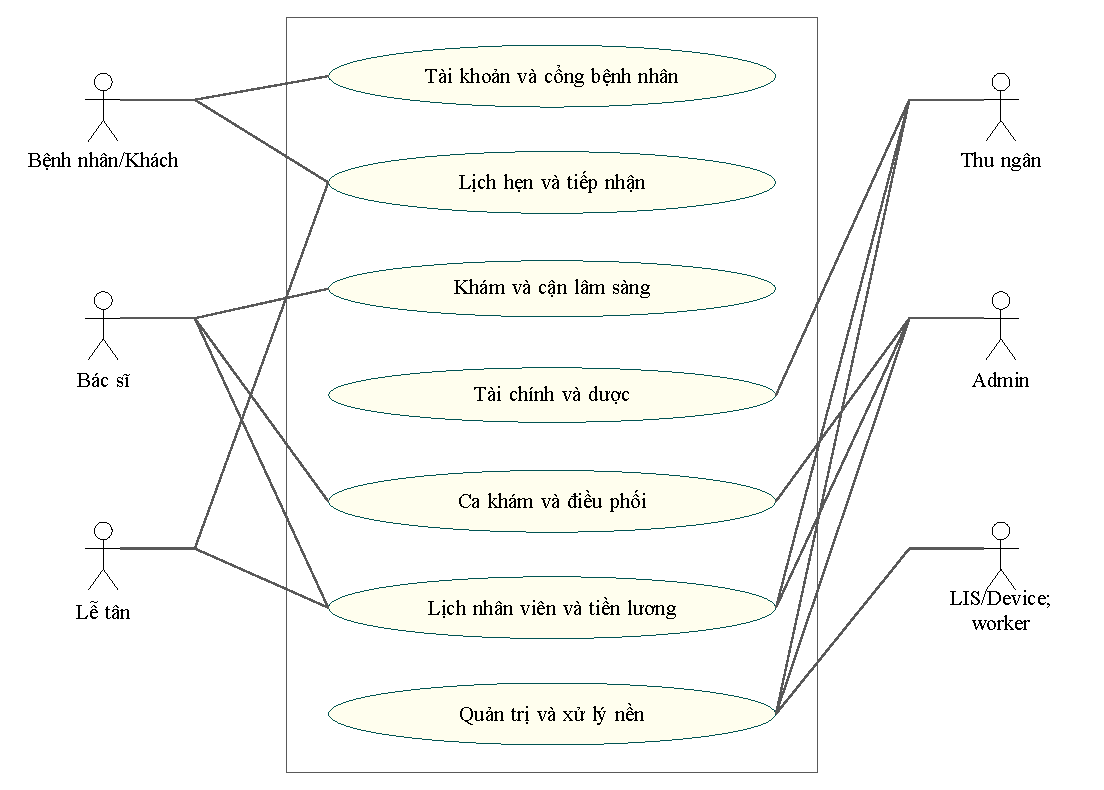
\includegraphics[width=1\textwidth,height=.61\textheight,keepaspectratio]{figures/diagrams/uc_overview.pdf}\captionof{figure}{Use case tổng quan hệ thống An Tâm}\label{fig:uc_overview}\end{center}
Sơ đồ tổng quan gom mục tiêu theo phân hệ để giữ khả năng đọc.\allowbreak{} Bảy nhóm được phân rã thành các sơ đồ tiếp theo.\allowbreak{} Nhân sự có quyền nhập/\allowbreak{}duyệt kết quả hoặc cấp phát không phải role mới; họ xuất hiện ở sơ đồ chi tiết theo permission bổ sung.\allowbreak{}

\clearpage

\Needspace{6\baselineskip}\subsection{Use case nhóm 1:\allowbreak{} tài khoản và cổng bệnh nhân}
\begin{center}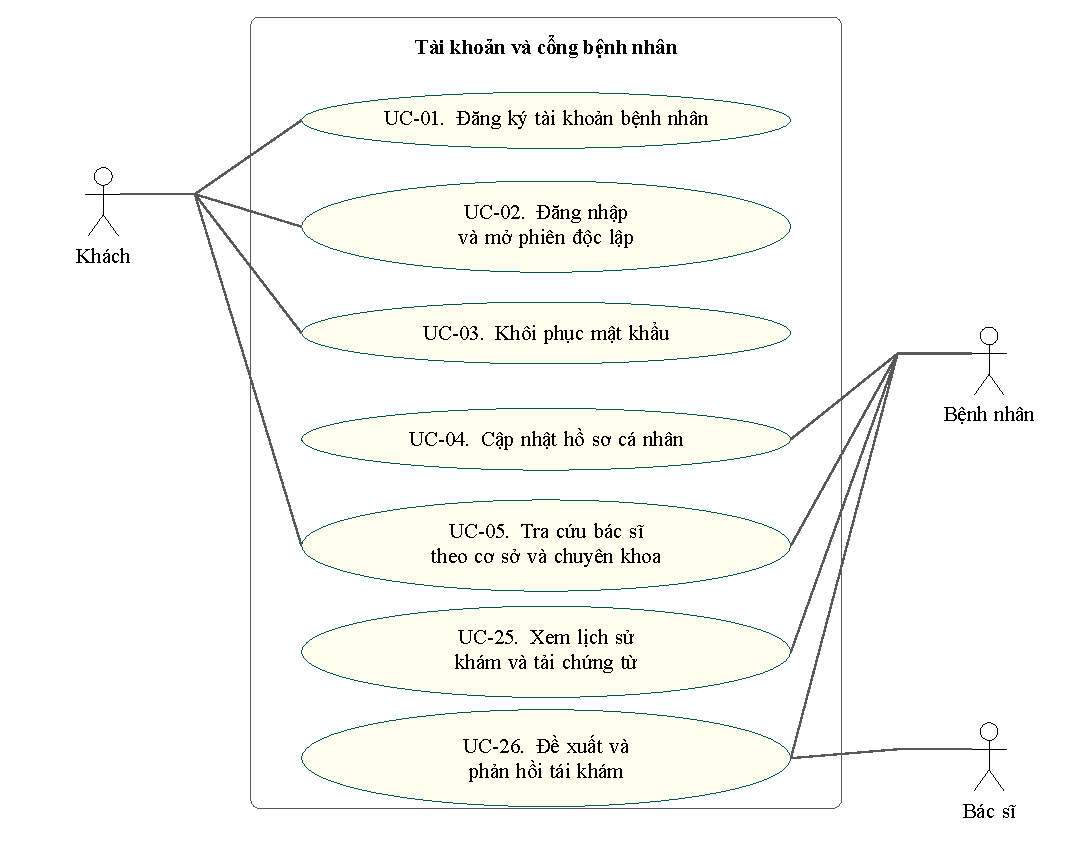
\includegraphics[width=1\textwidth,height=.61\textheight,keepaspectratio]{figures/diagrams/uc_g1.pdf}\captionof{figure}{Use case nhóm 1:\allowbreak{} tài khoản và cổng bệnh nhân}\label{fig:uc_g1}\end{center}
Đường nối là quan hệ tham gia giữa tác nhân và mục tiêu sử dụng.\allowbreak{} Các quyền chi tiết vẫn cần kiểm theo cơ sở; một vai trò trong sơ đồ không được mặc định truy cập mọi tài nguyên.\allowbreak{} Các mã UC dẫn tới đặc tả chi tiết ở phần sau.\allowbreak{}

\clearpage

\Needspace{6\baselineskip}\subsection{Use case nhóm 2:\allowbreak{} lịch hẹn và tiếp nhận}
\begin{center}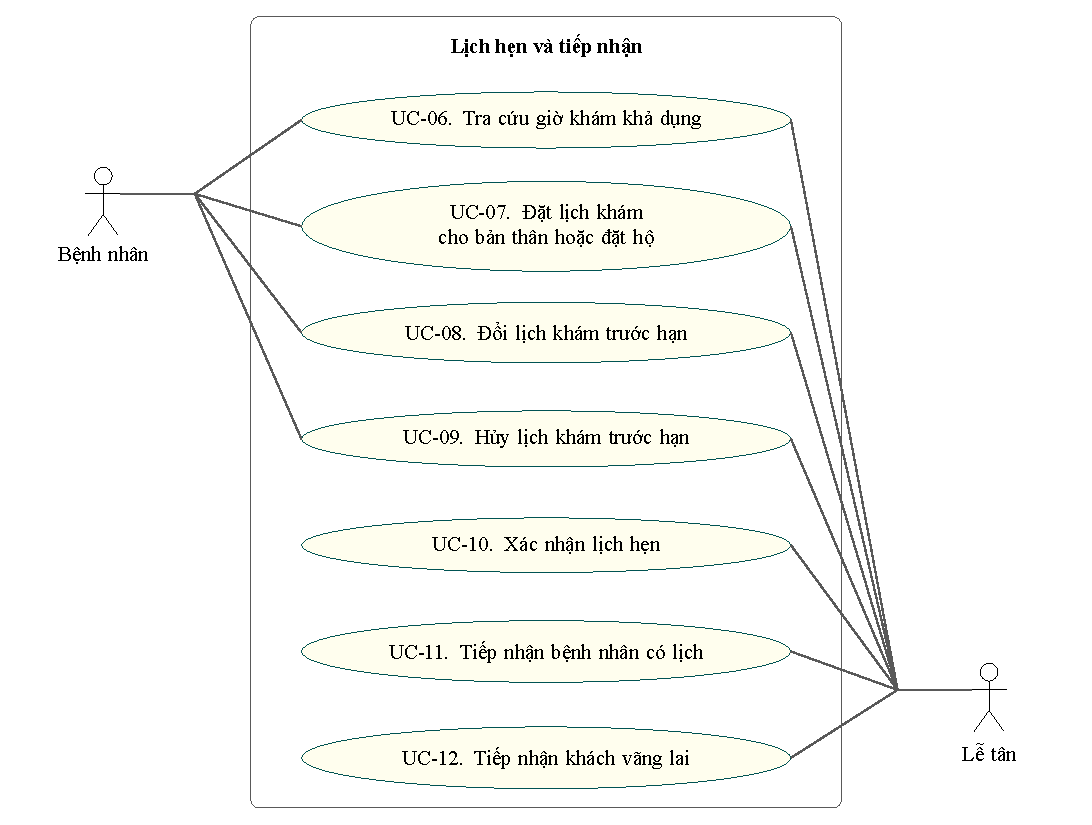
\includegraphics[width=1\textwidth,height=.61\textheight,keepaspectratio]{figures/diagrams/uc_g2.pdf}\captionof{figure}{Use case nhóm 2:\allowbreak{} lịch hẹn và tiếp nhận}\label{fig:uc_g2}\end{center}
Đường nối là quan hệ tham gia giữa tác nhân và mục tiêu sử dụng.\allowbreak{} Các quyền chi tiết vẫn cần kiểm theo cơ sở; một vai trò trong sơ đồ không được mặc định truy cập mọi tài nguyên.\allowbreak{} Các mã UC dẫn tới đặc tả chi tiết ở phần sau.\allowbreak{}

\clearpage

\Needspace{6\baselineskip}\subsection{Use case nhóm 3:\allowbreak{} khám và cận lâm sàng}
\begin{center}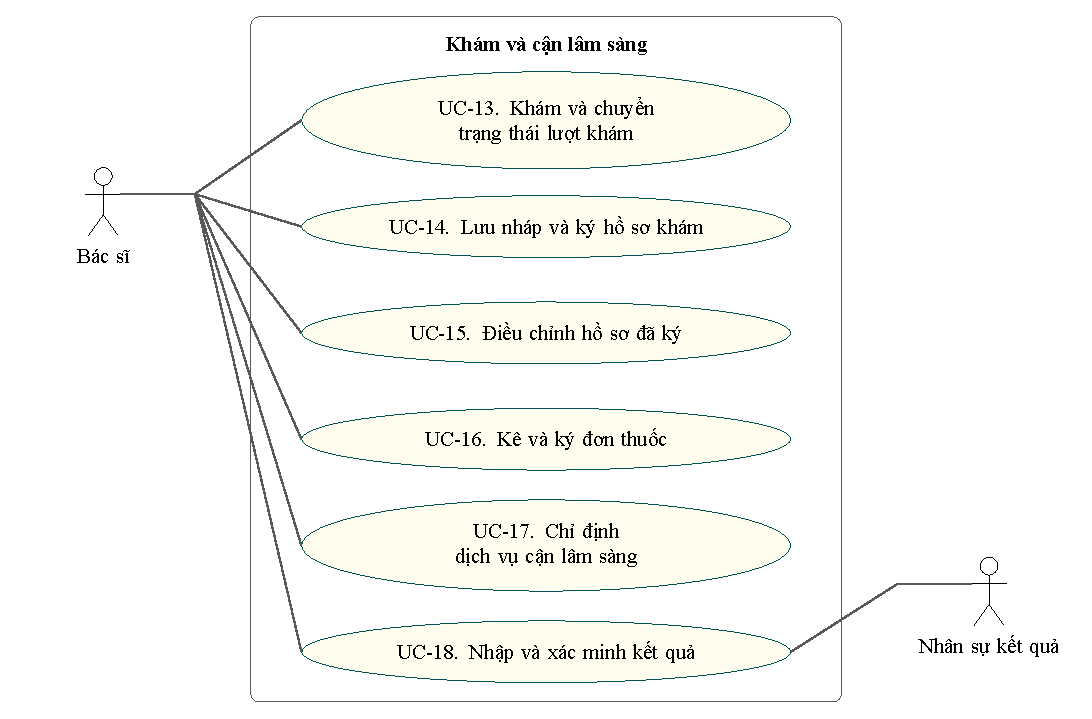
\includegraphics[width=1\textwidth,height=.61\textheight,keepaspectratio]{figures/diagrams/uc_g3.pdf}\captionof{figure}{Use case nhóm 3:\allowbreak{} khám và cận lâm sàng}\label{fig:uc_g3}\end{center}
Đường nối là quan hệ tham gia giữa tác nhân và mục tiêu sử dụng.\allowbreak{} Các quyền chi tiết vẫn cần kiểm theo cơ sở; một vai trò trong sơ đồ không được mặc định truy cập mọi tài nguyên.\allowbreak{} Các mã UC dẫn tới đặc tả chi tiết ở phần sau.\allowbreak{}

\clearpage

\Needspace{6\baselineskip}\subsection{Use case nhóm 4:\allowbreak{} tài chính và dược}
\begin{center}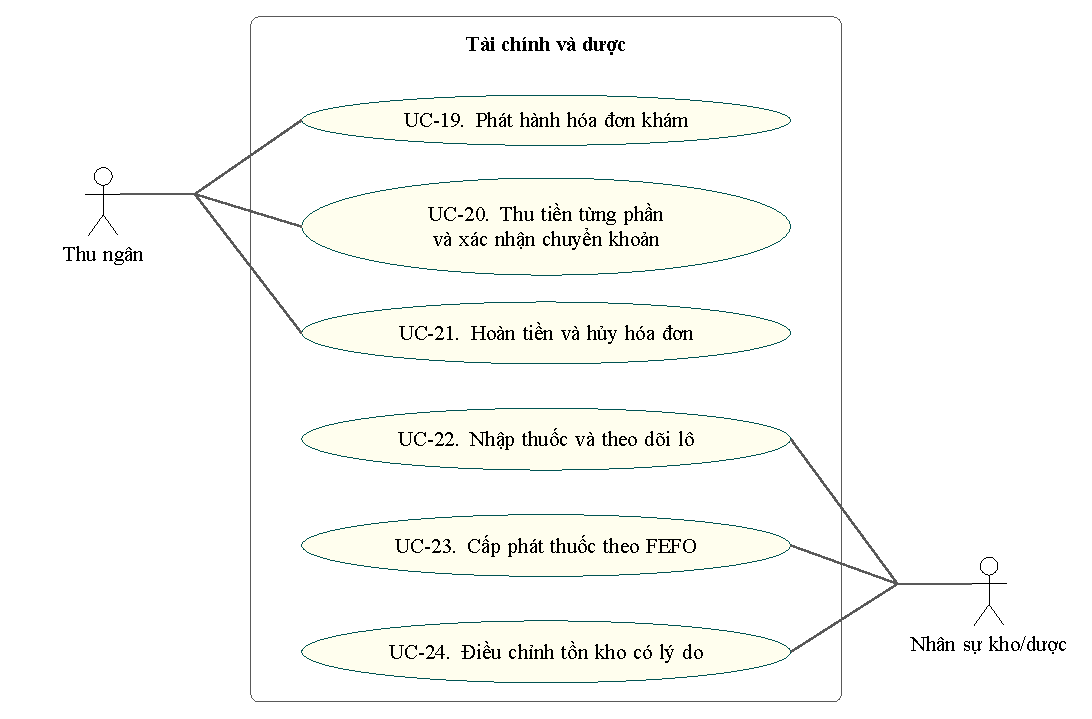
\includegraphics[width=1\textwidth,height=.61\textheight,keepaspectratio]{figures/diagrams/uc_g4.pdf}\captionof{figure}{Use case nhóm 4:\allowbreak{} tài chính và dược}\label{fig:uc_g4}\end{center}
Đường nối là quan hệ tham gia giữa tác nhân và mục tiêu sử dụng.\allowbreak{} Các quyền chi tiết vẫn cần kiểm theo cơ sở; một vai trò trong sơ đồ không được mặc định truy cập mọi tài nguyên.\allowbreak{} Các mã UC dẫn tới đặc tả chi tiết ở phần sau.\allowbreak{}

\clearpage

\Needspace{6\baselineskip}\subsection{Use case nhóm 5:\allowbreak{} ca khám và điều phối}
\begin{center}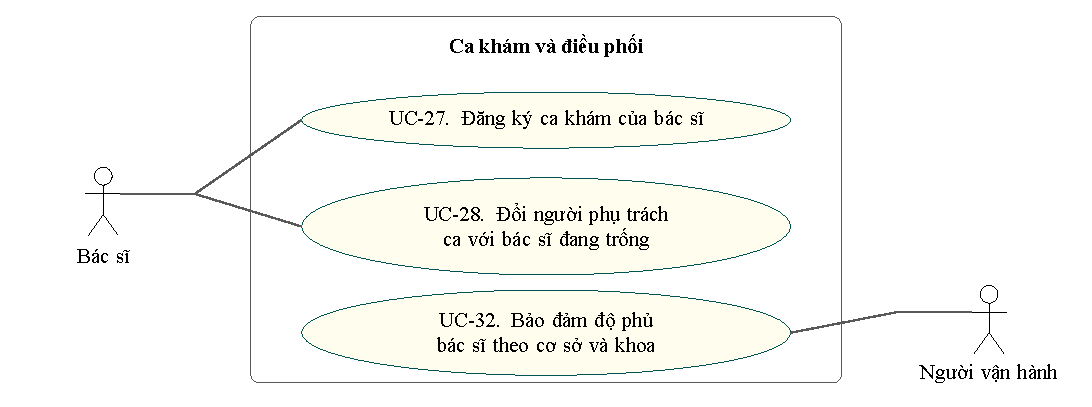
\includegraphics[width=1\textwidth,height=.61\textheight,keepaspectratio]{figures/diagrams/uc_g5.pdf}\captionof{figure}{Use case nhóm 5:\allowbreak{} ca khám và điều phối}\label{fig:uc_g5}\end{center}
Đường nối là quan hệ tham gia giữa tác nhân và mục tiêu sử dụng.\allowbreak{} Các quyền chi tiết vẫn cần kiểm theo cơ sở; một vai trò trong sơ đồ không được mặc định truy cập mọi tài nguyên.\allowbreak{} Các mã UC dẫn tới đặc tả chi tiết ở phần sau.\allowbreak{}

\clearpage

\Needspace{6\baselineskip}\subsection{Use case nhóm 6:\allowbreak{} lịch nhân viên và tiền lương}
\begin{center}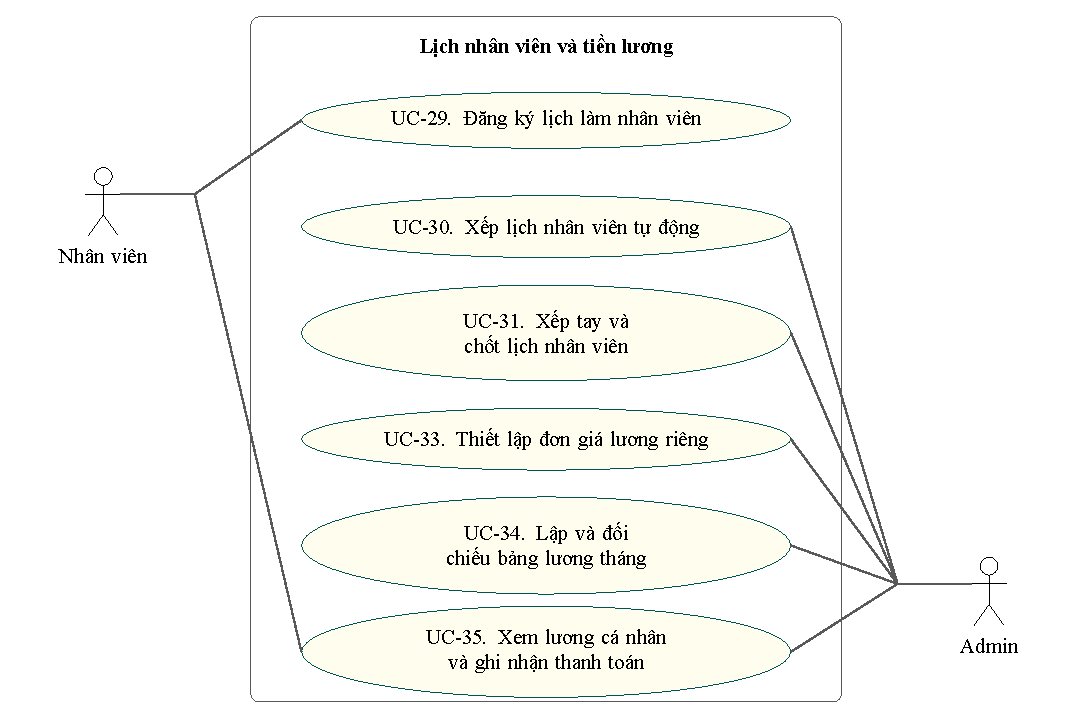
\includegraphics[width=1\textwidth,height=.61\textheight,keepaspectratio]{figures/diagrams/uc_g6.pdf}\captionof{figure}{Use case nhóm 6:\allowbreak{} lịch nhân viên và tiền lương}\label{fig:uc_g6}\end{center}
Đường nối là quan hệ tham gia giữa tác nhân và mục tiêu sử dụng.\allowbreak{} Các quyền chi tiết vẫn cần kiểm theo cơ sở; một vai trò trong sơ đồ không được mặc định truy cập mọi tài nguyên.\allowbreak{} Các mã UC dẫn tới đặc tả chi tiết ở phần sau.\allowbreak{}

\clearpage

\Needspace{6\baselineskip}\subsection{Use case nhóm 7:\allowbreak{} quản trị và xử lý nền}
\begin{center}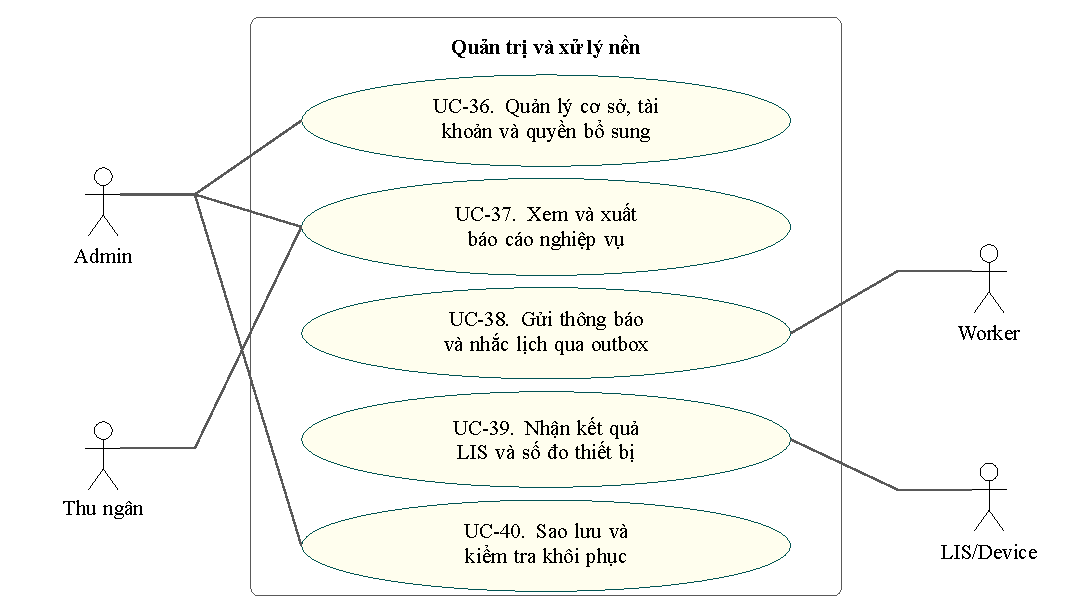
\includegraphics[width=1\textwidth,height=.61\textheight,keepaspectratio]{figures/diagrams/uc_g7.pdf}\captionof{figure}{Use case nhóm 7:\allowbreak{} quản trị và xử lý nền}\label{fig:uc_g7}\end{center}
Đường nối là quan hệ tham gia giữa tác nhân và mục tiêu sử dụng.\allowbreak{} Các quyền chi tiết vẫn cần kiểm theo cơ sở; một vai trò trong sơ đồ không được mặc định truy cập mọi tài nguyên.\allowbreak{} Các mã UC dẫn tới đặc tả chi tiết ở phần sau.\allowbreak{}

\clearpage

\section{Đặc tả chi tiết các use case}

\Needspace{6\baselineskip}\subsection{UC-01.\allowbreak{} Đăng ký tài khoản bệnh nhân}
\label{uc:1}

{\small\setlength{\tabcolsep}{3pt}\renewcommand{\arraystretch}{1.12}
\begin{longtable}{@{}L{\dimexpr 0.22\textwidth-1.32pt\relax} L{\dimexpr 0.78\textwidth-4.68pt\relax}@{}}
\caption{Đặc tả UC-01}\\
\toprule
\textbf{Thuộc tính} & \textbf{Đặc tả}\\\midrule
\endfirsthead
\toprule
\textbf{Thuộc tính} & \textbf{Đặc tả}\\\midrule
\endhead
\bottomrule\endlastfoot
Tác nhân & Khách chưa đăng nhập\\[3pt]
Mục tiêu & Đăng ký tài khoản bệnh nhân\\[3pt]
Điều kiện bắt đầu & Email chưa được sử dụng; dữ liệu đăng ký hợp lệ; người gửi chưa có phiên đăng nhập.\allowbreak{}\\[3pt]
Hậu điều kiện & Có tài khoản bệnh nhân liên kết hồ sơ; mật khẩu không được lưu ở dạng rõ.\allowbreak{}\\[3pt]
\end{longtable}}
\noindent\textbf{Luồng thành công chính.}
\begin{enumerate}
\item Khách mở trang đăng ký và nhập họ tên, email, mật khẩu cùng thông tin liên hệ.\allowbreak{}
\item Máy chủ kiểm tra dữ liệu, tính duy nhất của email và giới hạn tần suất.\allowbreak{}
\item Hệ thống băm mật khẩu, tạo tài khoản vai trò patient và hồ sơ bệnh nhân có mã riêng.\allowbreak{}
\item Phiên được thiết lập để bệnh nhân tiếp tục xem hồ sơ và đặt lịch.\allowbreak{}
\end{enumerate}
\noindent\textbf{Luồng thay thế và ngoại lệ.}
\begin{enumerate}
\item Email đã tồn tại:\allowbreak{} trả lỗi tại trường email, không tạo hồ sơ thứ hai.\allowbreak{}
\item Dữ liệu thiếu hoặc mật khẩu xác nhận không khớp:\allowbreak{} giữ các trường an toàn và yêu cầu sửa.\allowbreak{}
\end{enumerate}
Quy tắc trọng tâm:\allowbreak{} Vai trò đăng ký công khai luôn là patient; tham số vai trò từ trình duyệt không cấp quyền nhân viên.\allowbreak{}

\clearpage

\Needspace{6\baselineskip}\subsection{UC-02.\allowbreak{} Đăng nhập và mở phiên độc lập}
\label{uc:2}

{\small\setlength{\tabcolsep}{3pt}\renewcommand{\arraystretch}{1.12}
\begin{longtable}{@{}L{\dimexpr 0.22\textwidth-1.32pt\relax} L{\dimexpr 0.78\textwidth-4.68pt\relax}@{}}
\caption{Đặc tả UC-02}\\
\toprule
\textbf{Thuộc tính} & \textbf{Đặc tả}\\\midrule
\endfirsthead
\toprule
\textbf{Thuộc tính} & \textbf{Đặc tả}\\\midrule
\endhead
\bottomrule\endlastfoot
Tác nhân & Người dùng\\[3pt]
Mục tiêu & Đăng nhập và mở phiên độc lập\\[3pt]
Điều kiện bắt đầu & Tài khoản đang hoạt động; đúng thông tin đăng nhập; cookie và session sử dụng được.\allowbreak{}\\[3pt]
Hậu điều kiện & Phiên hiện tại gắn đúng người dùng; phiên local khác không thay thế tài khoản ở tab trước.\allowbreak{}\\[3pt]
\end{longtable}}
\noindent\textbf{Luồng thành công chính.}
\begin{enumerate}
\item Người dùng nhập email và mật khẩu tại biểu mẫu có CSRF token.\allowbreak{}
\item Hệ thống xác thực, kiểm tra trạng thái tài khoản và tái tạo phiên.\allowbreak{}
\item Người dùng được chuyển tới Thông báo theo quyền hiện tại.\allowbreak{}
\item Nếu cần dùng thêm tài khoản trong cùng cửa sổ, người dùng mở liên kết phiên riêng ở menu tài khoản.\allowbreak{}
\item Ứng dụng tạo hostname localhost riêng để cookie các tài khoản không dùng chung.\allowbreak{}
\end{enumerate}
\noindent\textbf{Luồng thay thế và ngoại lệ.}
\begin{enumerate}
\item Sai mật khẩu hoặc tài khoản khóa:\allowbreak{} phản hồi chung, không tiết lộ chi tiết tài khoản.\allowbreak{}
\item Đăng nhập từ trang quá hạn:\allowbreak{} mở lại biểu mẫu mới; không phát lại mật khẩu đã gửi.\allowbreak{}
\item Hostname bên ngoài hoặc production:\allowbreak{} không bật tiện ích phiên local độc lập.\allowbreak{}
\end{enumerate}
Quy tắc trọng tâm:\allowbreak{} Không truyền mật khẩu hoặc token đăng nhập trong URL; CSRF vẫn được giữ.\allowbreak{}

\clearpage

\Needspace{6\baselineskip}\subsection{UC-03.\allowbreak{} Khôi phục mật khẩu}
\label{uc:3}

{\small\setlength{\tabcolsep}{3pt}\renewcommand{\arraystretch}{1.12}
\begin{longtable}{@{}L{\dimexpr 0.22\textwidth-1.32pt\relax} L{\dimexpr 0.78\textwidth-4.68pt\relax}@{}}
\caption{Đặc tả UC-03}\\
\toprule
\textbf{Thuộc tính} & \textbf{Đặc tả}\\\midrule
\endfirsthead
\toprule
\textbf{Thuộc tính} & \textbf{Đặc tả}\\\midrule
\endhead
\bottomrule\endlastfoot
Tác nhân & Người dùng quên mật khẩu\\[3pt]
Mục tiêu & Khôi phục mật khẩu\\[3pt]
Điều kiện bắt đầu & Người dùng truy cập trang quên mật khẩu; có kênh email được cấu hình để nhận liên kết.\allowbreak{}\\[3pt]
Hậu điều kiện & Mật khẩu mới có hiệu lực khi token hợp lệ; token dùng một lần.\allowbreak{}\\[3pt]
\end{longtable}}
\noindent\textbf{Luồng thành công chính.}
\begin{enumerate}
\item Nhập địa chỉ email và gửi yêu cầu khôi phục.\allowbreak{}
\item Ứng dụng áp dụng giới hạn riêng cho nhóm khôi phục mật khẩu.\allowbreak{}
\item Nếu email hợp lệ trong hệ thống, tạo token và gửi liên kết; phản hồi bên ngoài vẫn thống nhất.\allowbreak{}
\item Người dùng mở liên kết, nhập mật khẩu mới và xác nhận.\allowbreak{}
\item Hệ thống kiểm tra thời hạn, cập nhật giá trị băm và làm token mất hiệu lực.\allowbreak{}
\end{enumerate}
\noindent\textbf{Luồng thay thế và ngoại lệ.}
\begin{enumerate}
\item Gửi quá nhanh:\allowbreak{} hiện thời gian cần đợi trên biểu mẫu; JSON nhận 429 và thời gian thử lại.\allowbreak{}
\item Token quá hạn hoặc đã dùng:\allowbreak{} không đổi mật khẩu.\allowbreak{}
\item MAIL\_\allowbreak{}MAILER=log:\allowbreak{} nội dung thư được ghi log, chưa giao đến hộp thư bên ngoài.\allowbreak{}
\end{enumerate}
Quy tắc trọng tâm:\allowbreak{} Liên kết hết hạn sau 60 phút theo cấu hình; không cho biết email có tồn tại qua thông báo xác nhận.\allowbreak{}

\clearpage

\Needspace{6\baselineskip}\subsection{UC-04.\allowbreak{} Cập nhật hồ sơ cá nhân}
\label{uc:4}

{\small\setlength{\tabcolsep}{3pt}\renewcommand{\arraystretch}{1.12}
\begin{longtable}{@{}L{\dimexpr 0.22\textwidth-1.32pt\relax} L{\dimexpr 0.78\textwidth-4.68pt\relax}@{}}
\caption{Đặc tả UC-04}\\
\toprule
\textbf{Thuộc tính} & \textbf{Đặc tả}\\\midrule
\endfirsthead
\toprule
\textbf{Thuộc tính} & \textbf{Đặc tả}\\\midrule
\endhead
\bottomrule\endlastfoot
Tác nhân & Bệnh nhân\\[3pt]
Mục tiêu & Cập nhật hồ sơ cá nhân\\[3pt]
Điều kiện bắt đầu & Bệnh nhân đăng nhập và có hồ sơ liên kết với tài khoản.\allowbreak{}\\[3pt]
Hậu điều kiện & Hồ sơ cá nhân được cập nhật; lịch khám và chứng từ đã phát hành không bị đổi chủ.\allowbreak{}\\[3pt]
\end{longtable}}
\noindent\textbf{Luồng thành công chính.}
\begin{enumerate}
\item Bệnh nhân mở Hồ sơ và xem thông tin đang lưu.\allowbreak{}
\item Sửa những trường được phép, gồm thông tin liên hệ, dị ứng hoặc tiền sử.\allowbreak{}
\item Máy chủ xác thực dữ liệu và xác định hồ sơ từ phiên đăng nhập.\allowbreak{}
\item Hệ thống cập nhật hồ sơ và phản hồi thành công.\allowbreak{}
\end{enumerate}
\noindent\textbf{Luồng thay thế và ngoại lệ.}
\begin{enumerate}
\item Gửi mã hồ sơ người khác:\allowbreak{} không thay đổi chủ thể cập nhật.\allowbreak{}
\item Dữ liệu không hợp lệ:\allowbreak{} trả lỗi và giữ dữ liệu hợp lệ để nhập lại.\allowbreak{}
\end{enumerate}
Quy tắc trọng tâm:\allowbreak{} Chủ thể hồ sơ lấy từ user hiện tại; không dùng patient\_\allowbreak{}id tùy ý để vượt quyền.\allowbreak{}

\clearpage

\Needspace{6\baselineskip}\subsection{UC-05.\allowbreak{} Tra cứu bác sĩ theo cơ sở và chuyên khoa}
\label{uc:5}

{\small\setlength{\tabcolsep}{3pt}\renewcommand{\arraystretch}{1.12}
\begin{longtable}{@{}L{\dimexpr 0.22\textwidth-1.32pt\relax} L{\dimexpr 0.78\textwidth-4.68pt\relax}@{}}
\caption{Đặc tả UC-05}\\
\toprule
\textbf{Thuộc tính} & \textbf{Đặc tả}\\\midrule
\endfirsthead
\toprule
\textbf{Thuộc tính} & \textbf{Đặc tả}\\\midrule
\endhead
\bottomrule\endlastfoot
Tác nhân & Khách; Bệnh nhân; Nhân viên\\[3pt]
Mục tiêu & Tra cứu bác sĩ theo cơ sở và chuyên khoa\\[3pt]
Điều kiện bắt đầu & Bác sĩ, chuyên khoa và cơ sở cần tra cứu đang hoạt động.\allowbreak{}\\[3pt]
Hậu điều kiện & Danh sách trả về đúng bộ lọc, không công bố dữ liệu bệnh nhân.\allowbreak{}\\[3pt]
\end{longtable}}
\noindent\textbf{Luồng thành công chính.}
\begin{enumerate}
\item Mở danh sách Bác sĩ.\allowbreak{}
\item Chọn cơ sở và chuyên khoa rồi thực hiện tra cứu.\allowbreak{}
\item Ứng dụng tải thông tin bác sĩ cùng chuyên khoa và phân công cơ sở.\allowbreak{}
\item Người dùng mở trang chi tiết để xem thông tin và lịch làm được công bố.\allowbreak{}
\item Phân trang tiếp tục giữ các điều kiện lọc.\allowbreak{}
\end{enumerate}
\noindent\textbf{Luồng thay thế và ngoại lệ.}
\begin{enumerate}
\item Không có bác sĩ phù hợp:\allowbreak{} hiển thị trạng thái rỗng.\allowbreak{}
\item Chi tiết không còn công bố:\allowbreak{} không hiển thị dữ liệu nội bộ thay thế.\allowbreak{}
\end{enumerate}
Quy tắc trọng tâm:\allowbreak{} Bác sĩ xuất hiện ở một cơ sở khi có phân công; danh sách chọn trên lịch được nhóm theo cơ sở.\allowbreak{}

\clearpage

\Needspace{6\baselineskip}\subsection{UC-06.\allowbreak{} Tra cứu giờ khám khả dụng}
\label{uc:6}

{\small\setlength{\tabcolsep}{3pt}\renewcommand{\arraystretch}{1.12}
\begin{longtable}{@{}L{\dimexpr 0.22\textwidth-1.32pt\relax} L{\dimexpr 0.78\textwidth-4.68pt\relax}@{}}
\caption{Đặc tả UC-06}\\
\toprule
\textbf{Thuộc tính} & \textbf{Đặc tả}\\\midrule
\endfirsthead
\toprule
\textbf{Thuộc tính} & \textbf{Đặc tả}\\\midrule
\endhead
\bottomrule\endlastfoot
Tác nhân & Bệnh nhân; Lễ tân\\[3pt]
Mục tiêu & Tra cứu giờ khám khả dụng\\[3pt]
Điều kiện bắt đầu & Đã chọn bác sĩ, cơ sở và ngày khám; bác sĩ có phân công hoạt động tại cơ sở.\allowbreak{}\\[3pt]
Hậu điều kiện & Danh sách giờ chỉ là ảnh chụp khả dụng; đặt lịch phải kiểm tra lại trong giao dịch.\allowbreak{}\\[3pt]
\end{longtable}}
\noindent\textbf{Luồng thành công chính.}
\begin{enumerate}
\item Ứng dụng lấy các ca đang mở trong ngày tại cơ sở đã chọn.\allowbreak{}
\item Chia ca thành các khoảng đủ slot\_\allowbreak{}minutes, không vượt cuối ca.\allowbreak{}
\item Loại bỏ khoảng đã qua và khoảng giao với lịch nghỉ bác sĩ.\allowbreak{}
\item Đếm lịch hiệu lực giao với từng khoảng theo bác sĩ trên toàn bộ cơ sở.\allowbreak{}
\item Trả giờ bắt đầu, kết thúc và sức chứa còn lại để chọn.\allowbreak{}
\end{enumerate}
\noindent\textbf{Luồng thay thế và ngoại lệ.}
\begin{enumerate}
\item Không có ca hoặc ca đóng:\allowbreak{} danh sách giờ rỗng.\allowbreak{}
\item Ca hết chỗ:\allowbreak{} loại giờ đó khỏi kết quả.\allowbreak{}
\item Đổi bộ lọc khi yêu cầu cũ chưa xong:\allowbreak{} giao diện cần sử dụng kết quả của lựa chọn hiện tại.\allowbreak{}
\end{enumerate}
Quy tắc trọng tâm:\allowbreak{} CANCELLED và NO\_\allowbreak{}SHOW không chiếm chỗ; ca phải đủ trọn thời lượng khám.\allowbreak{}

\clearpage

\Needspace{6\baselineskip}\subsection{UC-07.\allowbreak{} Đặt lịch khám cho bản thân hoặc đặt hộ}
\label{uc:7}

{\small\setlength{\tabcolsep}{3pt}\renewcommand{\arraystretch}{1.12}
\begin{longtable}{@{}L{\dimexpr 0.22\textwidth-1.32pt\relax} L{\dimexpr 0.78\textwidth-4.68pt\relax}@{}}
\caption{Đặc tả UC-07}\\
\toprule
\textbf{Thuộc tính} & \textbf{Đặc tả}\\\midrule
\endfirsthead
\toprule
\textbf{Thuộc tính} & \textbf{Đặc tả}\\\midrule
\endhead
\bottomrule\endlastfoot
Tác nhân & Bệnh nhân; Lễ tân\\[3pt]
Mục tiêu & Đặt lịch khám cho bản thân hoặc đặt hộ\\[3pt]
Điều kiện bắt đầu & Bệnh nhân hoạt động; bác sĩ hoạt động và được phân công; có giờ trống tại cơ sở.\allowbreak{}\\[3pt]
Hậu điều kiện & Một lịch hợp lệ được lưu, không tạo hai lịch vì bấm gửi lặp.\allowbreak{}\\[3pt]
\end{longtable}}
\noindent\textbf{Luồng thành công chính.}
\begin{enumerate}
\item Chọn bệnh nhân nếu lễ tân đặt hộ; bệnh nhân tự đặt dùng hồ sơ của mình.\allowbreak{}
\item Chọn cơ sở, chuyên khoa, bác sĩ, ngày, giờ và nhập lý do khám.\allowbreak{}
\item Gửi yêu cầu kèm khóa idempotency\_\allowbreak{}key.\allowbreak{}
\item Dịch vụ khóa bác sĩ và bệnh nhân, đọc lại hồ sơ và kiểm tra khoảng giờ.\allowbreak{}
\item Tạo lịch trạng thái PENDING cùng liên kết ca; ghi outbox và audit.\allowbreak{}
\item Trả mã lịch để tra cứu và tiếp tục theo dõi.\allowbreak{}
\end{enumerate}
\noindent\textbf{Luồng thay thế và ngoại lệ.}
\begin{enumerate}
\item Giờ vừa hết chỗ hoặc bệnh nhân đã có lịch trùng:\allowbreak{} báo lỗi, không lưu một phần.\allowbreak{}
\item Gửi lại cùng khóa và cùng nội dung:\allowbreak{} trả lịch đã có.\allowbreak{}
\item Dùng khóa cũ với nội dung khác:\allowbreak{} trả xung đột 409.\allowbreak{}
\end{enumerate}
Quy tắc trọng tâm:\allowbreak{} Khả dụng được kiểm tra sau khi khóa; thao tác giao diện không quyết định sức chứa cuối cùng.\allowbreak{}

\clearpage

\Needspace{6\baselineskip}\subsection{UC-08.\allowbreak{} Đổi lịch khám trước hạn}
\label{uc:8}

{\small\setlength{\tabcolsep}{3pt}\renewcommand{\arraystretch}{1.12}
\begin{longtable}{@{}L{\dimexpr 0.22\textwidth-1.32pt\relax} L{\dimexpr 0.78\textwidth-4.68pt\relax}@{}}
\caption{Đặc tả UC-08}\\
\toprule
\textbf{Thuộc tính} & \textbf{Đặc tả}\\\midrule
\endfirsthead
\toprule
\textbf{Thuộc tính} & \textbf{Đặc tả}\\\midrule
\endhead
\bottomrule\endlastfoot
Tác nhân & Bệnh nhân; Lễ tân\\[3pt]
Mục tiêu & Đổi lịch khám trước hạn\\[3pt]
Điều kiện bắt đầu & Lịch PENDING hoặc CONFIRMED; người dùng có quyền; bệnh nhân còn ít nhất 24 giờ trước lịch cũ.\allowbreak{}\\[3pt]
Hậu điều kiện & Lịch có thời điểm mới và lịch sử cũ/\allowbreak{}mới; không làm mất mã lịch.\allowbreak{}\\[3pt]
\end{longtable}}
\noindent\textbf{Luồng thành công chính.}
\begin{enumerate}
\item Mở lịch cần đổi và xem hạn đổi/\allowbreak{}hủy.\allowbreak{}
\item Chọn ngày, giờ mới của cùng bác sĩ và cùng cơ sở; nhập lý do.\allowbreak{}
\item Dịch vụ khóa bác sĩ, lịch và bệnh nhân; kiểm tra lại chủ thể cùng trạng thái.\allowbreak{}
\item Nếu người thực hiện là bệnh nhân, kiểm tra hạn dựa trên giờ khám cũ.\allowbreak{}
\item Kiểm tra slot mới, cập nhật lịch và ghi appointment\_\allowbreak{}history.\allowbreak{}
\item Hủy nhắc cũ, tạo thông báo lịch đổi và phản hồi thành công.\allowbreak{}
\end{enumerate}
\noindent\textbf{Luồng thay thế và ngoại lệ.}
\begin{enumerate}
\item Còn dưới 24 giờ:\allowbreak{} trả thông báo không thể đổi, giữ nguyên lịch.\allowbreak{}
\item Đúng 24 giờ:\allowbreak{} được phép nếu các điều kiện khác hợp lệ.\allowbreak{}
\item Bác sĩ phụ trách vừa thay đổi qua chuyển ca:\allowbreak{} yêu cầu tải lại trước khi tiếp tục.\allowbreak{}
\end{enumerate}
Quy tắc trọng tâm:\allowbreak{} Luồng đổi ngày/\allowbreak{}giờ hiện tại giữ bác sĩ và cơ sở, không phải chức năng chuyển khám liên cơ sở.\allowbreak{}

\clearpage

\Needspace{6\baselineskip}\subsection{UC-09.\allowbreak{} Hủy lịch khám trước hạn}
\label{uc:9}

{\small\setlength{\tabcolsep}{3pt}\renewcommand{\arraystretch}{1.12}
\begin{longtable}{@{}L{\dimexpr 0.22\textwidth-1.32pt\relax} L{\dimexpr 0.78\textwidth-4.68pt\relax}@{}}
\caption{Đặc tả UC-09}\\
\toprule
\textbf{Thuộc tính} & \textbf{Đặc tả}\\\midrule
\endfirsthead
\toprule
\textbf{Thuộc tính} & \textbf{Đặc tả}\\\midrule
\endhead
\bottomrule\endlastfoot
Tác nhân & Bệnh nhân; Lễ tân\\[3pt]
Mục tiêu & Hủy lịch khám trước hạn\\[3pt]
Điều kiện bắt đầu & Lịch còn PENDING hoặc CONFIRMED; bệnh nhân còn ít nhất 24 giờ nếu tự hủy.\allowbreak{}\\[3pt]
Hậu điều kiện & Lịch hủy được giữ để tra cứu; chỗ khám được giải phóng theo phép đếm lịch hiệu lực.\allowbreak{}\\[3pt]
\end{longtable}}
\noindent\textbf{Luồng thành công chính.}
\begin{enumerate}
\item Mở Lịch của tôi, nhập lý do hủy rồi xác nhận.\allowbreak{}
\item Máy chủ xác minh quyền và khóa bác sĩ, lịch đang xử lý.\allowbreak{}
\item Kiểm tra trạng thái và thời điểm giới hạn.\allowbreak{}
\item Cập nhật CANCELLED, cancel\_\allowbreak{}reason, cancelled\_\allowbreak{}at.\allowbreak{}
\item Hủy các nhắc chưa gửi, lưu thông báo hủy và nhật ký.\allowbreak{}
\end{enumerate}
\noindent\textbf{Luồng thay thế và ngoại lệ.}
\begin{enumerate}
\item Dưới mốc 24 giờ:\allowbreak{} hiện lỗi nghiệp vụ trong trang hiện tại thay cho trang debug.\allowbreak{}
\item Lịch đã tiếp nhận hoặc hoàn tất:\allowbreak{} không cho hủy qua luồng này.\allowbreak{}
\item Lịch đã đổi người phụ trách:\allowbreak{} báo tải lại để tránh ghi dựa dữ liệu cũ.\allowbreak{}
\end{enumerate}
Quy tắc trọng tâm:\allowbreak{} Không xóa lịch; thời điểm kiểm tra lấy từ máy chủ và múi giờ Việt Nam.\allowbreak{}

\clearpage

\Needspace{6\baselineskip}\subsection{UC-10.\allowbreak{} Xác nhận lịch hẹn}
\label{uc:10}

{\small\setlength{\tabcolsep}{3pt}\renewcommand{\arraystretch}{1.12}
\begin{longtable}{@{}L{\dimexpr 0.22\textwidth-1.32pt\relax} L{\dimexpr 0.78\textwidth-4.68pt\relax}@{}}
\caption{Đặc tả UC-10}\\
\toprule
\textbf{Thuộc tính} & \textbf{Đặc tả}\\\midrule
\endfirsthead
\toprule
\textbf{Thuộc tính} & \textbf{Đặc tả}\\\midrule
\endhead
\bottomrule\endlastfoot
Tác nhân & Lễ tân\\[3pt]
Mục tiêu & Xác nhận lịch hẹn\\[3pt]
Điều kiện bắt đầu & Lễ tân được phân công cơ sở; lịch đang PENDING.\allowbreak{}\\[3pt]
Hậu điều kiện & Lịch được xác nhận để tiếp nhận vào đúng ngày khám.\allowbreak{}\\[3pt]
\end{longtable}}
\noindent\textbf{Luồng thành công chính.}
\begin{enumerate}
\item Mở Thông báo hoặc chọn ca trên Quản lý thời gian.\allowbreak{}
\item Tìm lịch hẹn cần xác nhận theo mã, tên hoặc điện thoại.\allowbreak{}
\item Nhấn Xác nhận.\allowbreak{}
\item Máy chủ kiểm tra vai trò, cơ sở và trạng thái hiện tại.\allowbreak{}
\item Cập nhật CONFIRMED, ghi nhật ký và cập nhật nội dung hiển thị.\allowbreak{}
\end{enumerate}
\noindent\textbf{Luồng thay thế và ngoại lệ.}
\begin{enumerate}
\item Nhân viên cơ sở khác:\allowbreak{} từ chối 403.\allowbreak{}
\item Chuyển trạng thái không hợp lệ:\allowbreak{} phản hồi lỗi thân thiện với web, giữ 409 cho JSON.\allowbreak{}
\end{enumerate}
Quy tắc trọng tâm:\allowbreak{} Việc thấy một dòng lịch không tự tạo quyền xác nhận cho bác sĩ hoặc thu ngân.\allowbreak{}

\clearpage

\Needspace{6\baselineskip}\subsection{UC-11.\allowbreak{} Tiếp nhận bệnh nhân có lịch}
\label{uc:11}

{\small\setlength{\tabcolsep}{3pt}\renewcommand{\arraystretch}{1.12}
\begin{longtable}{@{}L{\dimexpr 0.22\textwidth-1.32pt\relax} L{\dimexpr 0.78\textwidth-4.68pt\relax}@{}}
\caption{Đặc tả UC-11}\\
\toprule
\textbf{Thuộc tính} & \textbf{Đặc tả}\\\midrule
\endfirsthead
\toprule
\textbf{Thuộc tính} & \textbf{Đặc tả}\\\midrule
\endhead
\bottomrule\endlastfoot
Tác nhân & Lễ tân\\[3pt]
Mục tiêu & Tiếp nhận bệnh nhân có lịch\\[3pt]
Điều kiện bắt đầu & Lịch CONFIRMED của ngày hiện tại; chưa có Visit; lễ tân có VISIT\_\allowbreak{}CHECK\_\allowbreak{}IN ở cơ sở.\allowbreak{}\\[3pt]
Hậu điều kiện & Một Visit gắn lịch hẹn, xuất hiện trong hàng chờ đúng bác sĩ.\allowbreak{}\\[3pt]
\end{longtable}}
\noindent\textbf{Luồng thành công chính.}
\begin{enumerate}
\item Lễ tân tìm lịch đã xác nhận và đối chiếu bệnh nhân đến khám.\allowbreak{}
\item Nhấn Tiếp nhận trên ca làm hoặc Thông báo.\allowbreak{}
\item Dịch vụ khóa bác sĩ và lịch, kiểm tra lại ngày khám, cơ sở và Visit hiện hữu.\allowbreak{}
\item Tạo Visit WAITING có mã lượt riêng và thời điểm tiếp nhận.\allowbreak{}
\item Đổi lịch sang CHECKED\_\allowbreak{}IN, hủy nhắc chưa gửi và ghi audit.\allowbreak{}
\end{enumerate}
\noindent\textbf{Luồng thay thế và ngoại lệ.}
\begin{enumerate}
\item Ngày tương lai hoặc quá ngày:\allowbreak{} không tiếp nhận qua thao tác này.\allowbreak{}
\item Bấm lần thứ hai:\allowbreak{} không tạo Visit trùng.\allowbreak{}
\item Bác sĩ đã được chuyển ca giữa lúc mở trang và gửi:\allowbreak{} yêu cầu tải lại.\allowbreak{}
\end{enumerate}
Quy tắc trọng tâm:\allowbreak{} Lịch hẹn và lượt khám là hai thực thể; mỗi lịch tối đa một Visit.\allowbreak{}

\clearpage

\Needspace{6\baselineskip}\subsection{UC-12.\allowbreak{} Tiếp nhận khách vãng lai}
\label{uc:12}

{\small\setlength{\tabcolsep}{3pt}\renewcommand{\arraystretch}{1.12}
\begin{longtable}{@{}L{\dimexpr 0.22\textwidth-1.32pt\relax} L{\dimexpr 0.78\textwidth-4.68pt\relax}@{}}
\caption{Đặc tả UC-12}\\
\toprule
\textbf{Thuộc tính} & \textbf{Đặc tả}\\\midrule
\endfirsthead
\toprule
\textbf{Thuộc tính} & \textbf{Đặc tả}\\\midrule
\endhead
\bottomrule\endlastfoot
Tác nhân & Lễ tân\\[3pt]
Mục tiêu & Tiếp nhận khách vãng lai\\[3pt]
Điều kiện bắt đầu & Có hồ sơ bệnh nhân và bác sĩ hoạt động tại cơ sở; lễ tân có quyền tiếp nhận.\allowbreak{}\\[3pt]
Hậu điều kiện & Có lượt khám độc lập, không sinh lịch hẹn giả để hợp thức hóa dữ liệu.\allowbreak{}\\[3pt]
\end{longtable}}
\noindent\textbf{Luồng thành công chính.}
\begin{enumerate}
\item Tìm hoặc tạo hồ sơ hành chính cho người đến trực tiếp.\allowbreak{}
\item Chọn bác sĩ, cơ sở và lý do khám.\allowbreak{}
\item Dịch vụ kiểm tra bệnh nhân, bác sĩ và phân công cơ sở.\allowbreak{}
\item Tạo Visit WAITING trực tiếp với appointment\_\allowbreak{}id rỗng.\allowbreak{}
\item Lượt xuất hiện tại màn hình Lượt khám của bác sĩ được giao.\allowbreak{}
\end{enumerate}
\noindent\textbf{Luồng thay thế và ngoại lệ.}
\begin{enumerate}
\item Hồ sơ ngừng hoạt động hoặc bác sĩ không thuộc cơ sở:\allowbreak{} từ chối.\allowbreak{}
\item Lễ tân chỉ có thể dùng cơ sở được cấp quyền.\allowbreak{}
\end{enumerate}
Quy tắc trọng tâm:\allowbreak{} Quan hệ Visit với Appointment là tùy chọn; khóa bệnh nhân vẫn là hồ sơ dùng chung.\allowbreak{}

\clearpage

\Needspace{6\baselineskip}\subsection{UC-13.\allowbreak{} Khám và chuyển trạng thái lượt khám}
\label{uc:13}

{\small\setlength{\tabcolsep}{3pt}\renewcommand{\arraystretch}{1.12}
\begin{longtable}{@{}L{\dimexpr 0.22\textwidth-1.32pt\relax} L{\dimexpr 0.78\textwidth-4.68pt\relax}@{}}
\caption{Đặc tả UC-13}\\
\toprule
\textbf{Thuộc tính} & \textbf{Đặc tả}\\\midrule
\endfirsthead
\toprule
\textbf{Thuộc tính} & \textbf{Đặc tả}\\\midrule
\endhead
\bottomrule\endlastfoot
Tác nhân & Bác sĩ phụ trách\\[3pt]
Mục tiêu & Khám và chuyển trạng thái lượt khám\\[3pt]
Điều kiện bắt đầu & Bác sĩ được giao Visit và có VISIT\_\allowbreak{}TREAT tại cơ sở.\allowbreak{}\\[3pt]
Hậu điều kiện & Lượt và các thời điểm phản ánh đúng tiến trình được phép.\allowbreak{}\\[3pt]
\end{longtable}}
\noindent\textbf{Luồng thành công chính.}
\begin{enumerate}
\item Mở hàng chờ của mình và bắt đầu lượt WAITING.\allowbreak{}
\item Ứng dụng chuyển IN\_\allowbreak{}PROGRESS và ghi started\_\allowbreak{}at lần đầu.\allowbreak{}
\item Bác sĩ có thể chuyển WAITING\_\allowbreak{}RESULT khi chờ cận lâm sàng, rồi quay lại khám.\allowbreak{}
\item Khi hoàn tất, máy chủ kiểm tra hồ sơ đã ký, không có đơn nháp hoặc chỉ định còn mở.\allowbreak{}
\item Chuyển COMPLETED và cập nhật lịch gốc nếu có; sau đó có thể đóng CLOSED.\allowbreak{}
\end{enumerate}
\noindent\textbf{Luồng thay thế và ngoại lệ.}
\begin{enumerate}
\item Chuyển trạng thái ngoài đồ thị:\allowbreak{} trả 409.\allowbreak{}
\item Còn đơn nháp hoặc kết quả chưa xong:\allowbreak{} từ chối hoàn tất với lỗi nghiệp vụ.\allowbreak{}
\item Bác sĩ khác hoặc admin không có quyền điều trị lượt đó:\allowbreak{} từ chối.\allowbreak{}
\end{enumerate}
Quy tắc trọng tâm:\allowbreak{} Quản trị hệ thống không đồng nghĩa với quyền điều trị; hoàn tất là điểm kiểm tra nhất quán chứng từ.\allowbreak{}

\clearpage

\Needspace{6\baselineskip}\subsection{UC-14.\allowbreak{} Lưu nháp và ký hồ sơ khám}
\label{uc:14}

{\small\setlength{\tabcolsep}{3pt}\renewcommand{\arraystretch}{1.12}
\begin{longtable}{@{}L{\dimexpr 0.22\textwidth-1.32pt\relax} L{\dimexpr 0.78\textwidth-4.68pt\relax}@{}}
\caption{Đặc tả UC-14}\\
\toprule
\textbf{Thuộc tính} & \textbf{Đặc tả}\\\midrule
\endfirsthead
\toprule
\textbf{Thuộc tính} & \textbf{Đặc tả}\\\midrule
\endhead
\bottomrule\endlastfoot
Tác nhân & Bác sĩ phụ trách\\[3pt]
Mục tiêu & Lưu nháp và ký hồ sơ khám\\[3pt]
Điều kiện bắt đầu & Visit IN\_\allowbreak{}PROGRESS hoặc WAITING\_\allowbreak{}RESULT; có quyền VISIT\_\allowbreak{}TREAT/\allowbreak{}RECORD\_\allowbreak{}SIGN tương ứng.\allowbreak{}\\[3pt]
Hậu điều kiện & Có hồ sơ DRAFT hoặc SIGNED gắn duy nhất Visit.\allowbreak{}\\[3pt]
\end{longtable}}
\noindent\textbf{Luồng thành công chính.}
\begin{enumerate}
\item Bác sĩ nhập triệu chứng, khám thực thể, chẩn đoán và kết luận.\allowbreak{}
\item Gửi cùng version đang đọc và hành động draft hoặc sign.\allowbreak{}
\item Máy chủ khóa Visit, đối chiếu phiên bản hồ sơ.\allowbreak{}
\item Lưu nội dung, tăng version; nếu ký thì ghi signed\_\allowbreak{}by, signed\_\allowbreak{}at và published\_\allowbreak{}at.\allowbreak{}
\item Ghi audit và trả hồ sơ mới để tiếp tục thao tác.\allowbreak{}
\end{enumerate}
\noindent\textbf{Luồng thay thế và ngoại lệ.}
\begin{enumerate}
\item Version cũ:\allowbreak{} trả xung đột, không ghi đè thay đổi ở phiên khác.\allowbreak{}
\item Hồ sơ đã ký:\allowbreak{} yêu cầu lý do điều chỉnh và lưu phiên bản cũ.\allowbreak{}
\end{enumerate}
Quy tắc trọng tâm:\allowbreak{} Ký trong ứng dụng là dấu vết nghiệp vụ, chưa phải chữ ký số PKI có chứng thư.\allowbreak{}

\clearpage

\Needspace{6\baselineskip}\subsection{UC-15.\allowbreak{} Điều chỉnh hồ sơ đã ký}
\label{uc:15}

{\small\setlength{\tabcolsep}{3pt}\renewcommand{\arraystretch}{1.12}
\begin{longtable}{@{}L{\dimexpr 0.22\textwidth-1.32pt\relax} L{\dimexpr 0.78\textwidth-4.68pt\relax}@{}}
\caption{Đặc tả UC-15}\\
\toprule
\textbf{Thuộc tính} & \textbf{Đặc tả}\\\midrule
\endfirsthead
\toprule
\textbf{Thuộc tính} & \textbf{Đặc tả}\\\midrule
\endhead
\bottomrule\endlastfoot
Tác nhân & Bác sĩ phụ trách\\[3pt]
Mục tiêu & Điều chỉnh hồ sơ đã ký\\[3pt]
Điều kiện bắt đầu & Hồ sơ SIGNED; đúng bác sĩ; có version mới nhất và lý do điều chỉnh.\allowbreak{}\\[3pt]
Hậu điều kiện & Lịch sử điều chỉnh được bảo toàn để đối chiếu nội dung trước và sau.\allowbreak{}\\[3pt]
\end{longtable}}
\noindent\textbf{Luồng thành công chính.}
\begin{enumerate}
\item Bác sĩ mở hồ sơ đã ký, đọc bản công bố hiện tại.\allowbreak{}
\item Nhập nội dung cần điều chỉnh cùng lý do; gửi hành động ký.\allowbreak{}
\item Dịch vụ kiểm tra version và điều kiện sửa lượt đã hoàn tất.\allowbreak{}
\item Chụp snapshot bản cũ vào medical\_\allowbreak{}record\_\allowbreak{}revisions kèm người sửa và lý do.\allowbreak{}
\item Lưu bản mới, tăng version và ghi lại thông tin ký.\allowbreak{}
\end{enumerate}
\noindent\textbf{Luồng thay thế và ngoại lệ.}
\begin{enumerate}
\item Thiếu lý do:\allowbreak{} từ chối thay đổi.\allowbreak{}
\item Hồ sơ ở lượt đóng chỉ nhận điều chỉnh đủ điều kiện, không quay về nháp tùy ý.\allowbreak{}
\end{enumerate}
Quy tắc trọng tâm:\allowbreak{} Không ghi đè mất dấu vết của hồ sơ đã ký; mỗi snapshot mang version nguồn.\allowbreak{}

\clearpage

\Needspace{6\baselineskip}\subsection{UC-16.\allowbreak{} Kê và ký đơn thuốc}
\label{uc:16}

{\small\setlength{\tabcolsep}{3pt}\renewcommand{\arraystretch}{1.12}
\begin{longtable}{@{}L{\dimexpr 0.22\textwidth-1.32pt\relax} L{\dimexpr 0.78\textwidth-4.68pt\relax}@{}}
\caption{Đặc tả UC-16}\\
\toprule
\textbf{Thuộc tính} & \textbf{Đặc tả}\\\midrule
\endfirsthead
\toprule
\textbf{Thuộc tính} & \textbf{Đặc tả}\\\midrule
\endhead
\bottomrule\endlastfoot
Tác nhân & Bác sĩ phụ trách\\[3pt]
Mục tiêu & Kê và ký đơn thuốc\\[3pt]
Điều kiện bắt đầu & Visit đang khám hoặc chờ kết quả; thuốc đang hoạt động; bác sĩ có quyền ký đơn.\allowbreak{}\\[3pt]
Hậu điều kiện & Đơn đã ký sẵn sàng xuất PDF hoặc cấp phát theo quyền.\allowbreak{}\\[3pt]
\end{longtable}}
\noindent\textbf{Luồng thành công chính.}
\begin{enumerate}
\item Chọn thuốc và nhập từng dòng liều dùng, đường dùng, tần suất, số ngày, số lượng.\allowbreak{}
\item Chọn có bán thuốc tại phòng khám hay chỉ kê đơn.\allowbreak{}
\item Ứng dụng tạo Prescription DRAFT và các Prescription\allowbreak{}Item.\allowbreak{}
\item Bác sĩ rà soát nội dung rồi ký.\allowbreak{}
\item Máy chủ kiểm tra đơn có dòng và lượt chưa đóng; cập nhật SIGNED cùng thông tin ký.\allowbreak{}
\end{enumerate}
\noindent\textbf{Luồng thay thế và ngoại lệ.}
\begin{enumerate}
\item Thuốc vô hiệu hóa:\allowbreak{} không thêm vào đơn mới.\allowbreak{}
\item Đơn rỗng hoặc đã ký:\allowbreak{} không ký lại qua cùng thao tác.\allowbreak{}
\item Lễ tân yêu cầu ký:\allowbreak{} bị từ chối ở máy chủ.\allowbreak{}
\end{enumerate}
Quy tắc trọng tâm:\allowbreak{} Ký đơn không giảm kho; cấp phát và thanh toán là các nghiệp vụ tách biệt.\allowbreak{}

\clearpage

\Needspace{6\baselineskip}\subsection{UC-17.\allowbreak{} Chỉ định dịch vụ cận lâm sàng}
\label{uc:17}

{\small\setlength{\tabcolsep}{3pt}\renewcommand{\arraystretch}{1.12}
\begin{longtable}{@{}L{\dimexpr 0.22\textwidth-1.32pt\relax} L{\dimexpr 0.78\textwidth-4.68pt\relax}@{}}
\caption{Đặc tả UC-17}\\
\toprule
\textbf{Thuộc tính} & \textbf{Đặc tả}\\\midrule
\endfirsthead
\toprule
\textbf{Thuộc tính} & \textbf{Đặc tả}\\\midrule
\endhead
\bottomrule\endlastfoot
Tác nhân & Bác sĩ phụ trách\\[3pt]
Mục tiêu & Chỉ định dịch vụ cận lâm sàng\\[3pt]
Điều kiện bắt đầu & Visit đang mở và chưa có hóa đơn; bác sĩ có SERVICE\_\allowbreak{}ORDER\_\allowbreak{}CREATE.\allowbreak{}\\[3pt]
Hậu điều kiện & Các dòng chỉ định có thể được nhập kết quả thủ công hoặc ánh xạ API.\allowbreak{}\\[3pt]
\end{longtable}}
\noindent\textbf{Luồng thành công chính.}
\begin{enumerate}
\item Chọn các dịch vụ cần chỉ định từ danh mục hoạt động.\allowbreak{}
\item Máy chủ loại các mã chọn trùng, kiểm tra quyền và khóa Visit.\allowbreak{}
\item Tạo Service\allowbreak{}Order gắn Visit và bác sĩ.\allowbreak{}
\item Tạo từng dòng chỉ định với external\_\allowbreak{}order\_\allowbreak{}code riêng.\allowbreak{}
\item Nhân sự có quyền kết quả nhận được các dòng tại màn hình Chẩn đoán.\allowbreak{}
\end{enumerate}
\noindent\textbf{Luồng thay thế và ngoại lệ.}
\begin{enumerate}
\item Dịch vụ ngừng hoạt động:\allowbreak{} từ chối.\allowbreak{}
\item Lượt hoặc hóa đơn đã chốt:\allowbreak{} không bổ sung chỉ định qua luồng hiện tại.\allowbreak{}
\end{enumerate}
Quy tắc trọng tâm:\allowbreak{} Mã chỉ định ngoài được dùng đối chiếu cùng patient/\allowbreak{}visit/\allowbreak{}branch, không tự đoán quan hệ.\allowbreak{}

\clearpage

\Needspace{6\baselineskip}\subsection{UC-18.\allowbreak{} Nhập và xác minh kết quả}
\label{uc:18}

{\small\setlength{\tabcolsep}{3pt}\renewcommand{\arraystretch}{1.12}
\begin{longtable}{@{}L{\dimexpr 0.22\textwidth-1.32pt\relax} L{\dimexpr 0.78\textwidth-4.68pt\relax}@{}}
\caption{Đặc tả UC-18}\\
\toprule
\textbf{Thuộc tính} & \textbf{Đặc tả}\\\midrule
\endfirsthead
\toprule
\textbf{Thuộc tính} & \textbf{Đặc tả}\\\midrule
\endhead
\bottomrule\endlastfoot
Tác nhân & Nhân sự được cấp quyền kết quả\\[3pt]
Mục tiêu & Nhập và xác minh kết quả\\[3pt]
Điều kiện bắt đầu & Có LAB\_\allowbreak{}RESULT\_\allowbreak{}ENTER hoặc LAB\_\allowbreak{}RESULT\_\allowbreak{}VERIFY tương ứng tại cơ sở của chỉ định.\allowbreak{}\\[3pt]
Hậu điều kiện & Chỉ kết quả đã xác minh mới được dùng cho công bố theo quyền.\allowbreak{}\\[3pt]
\end{longtable}}
\noindent\textbf{Luồng thành công chính.}
\begin{enumerate}
\item Nhập nội dung, đơn vị và tệp đính kèm tùy chọn cho dòng chỉ định.\allowbreak{}
\item Máy chủ kiểm tra định dạng/\allowbreak{}kích thước và lưu tệp trên disk local riêng.\allowbreak{}
\item Kết quả mới ở RECEIVED; dòng và phiếu chỉ định chuyển RESULT\_\allowbreak{}PENDING.\allowbreak{}
\item Người có quyền duyệt chọn VERIFIED hoặc REJECTED.\allowbreak{}
\item Khi tất cả dòng hợp lệ đã hoàn tất, hệ thống chuyển phiếu COMPLETED.\allowbreak{}
\end{enumerate}
\noindent\textbf{Luồng thay thế và ngoại lệ.}
\begin{enumerate}
\item Tệp quá 5 MB hoặc ngoài PDF/\allowbreak{}JPG/\allowbreak{}PNG:\allowbreak{} từ chối.\allowbreak{}
\item Dòng đã có kết quả VERIFIED:\allowbreak{} không duyệt thêm bản thứ hai.\allowbreak{}
\item Bệnh nhân chưa có kết quả được duyệt:\allowbreak{} không tải tệp chờ.\allowbreak{}
\end{enumerate}
Quy tắc trọng tâm:\allowbreak{} Quyền nhập và duyệt là quyền bổ sung, không cấp cho mọi bác sĩ hoặc admin một cách ngầm định.\allowbreak{}

\clearpage

\Needspace{6\baselineskip}\subsection{UC-19.\allowbreak{} Phát hành hóa đơn khám}
\label{uc:19}

{\small\setlength{\tabcolsep}{3pt}\renewcommand{\arraystretch}{1.12}
\begin{longtable}{@{}L{\dimexpr 0.22\textwidth-1.32pt\relax} L{\dimexpr 0.78\textwidth-4.68pt\relax}@{}}
\caption{Đặc tả UC-19}\\
\toprule
\textbf{Thuộc tính} & \textbf{Đặc tả}\\\midrule
\endfirsthead
\toprule
\textbf{Thuộc tính} & \textbf{Đặc tả}\\\midrule
\endhead
\bottomrule\endlastfoot
Tác nhân & Thu ngân có quyền tại cơ sở\\[3pt]
Mục tiêu & Phát hành hóa đơn khám\\[3pt]
Điều kiện bắt đầu & Visit COMPLETED hoặc CLOSED; chưa có hóa đơn chính; có INVOICE\_\allowbreak{}ISSUE.\allowbreak{}\\[3pt]
Hậu điều kiện & Hóa đơn lưu giá tại thời điểm phát hành, không đổi khi danh mục thay giá.\allowbreak{}\\[3pt]
\end{longtable}}
\noindent\textbf{Luồng thành công chính.}
\begin{enumerate}
\item Thu ngân mở lượt khám đã hoàn tất.\allowbreak{}
\item Hệ thống tổng hợp phí khám, dịch vụ hoàn tất và thuốc đã ký được đánh dấu bán.\allowbreak{}
\item Thu ngân nhập giảm giá và lý do nếu có.\allowbreak{}
\item Dịch vụ khóa Visit, tạo Invoice ISSUED và các dòng snapshot đơn giá, mô tả, nguồn.\allowbreak{}
\item Tính subtotal, discount, total rồi ghi audit.\allowbreak{}
\end{enumerate}
\noindent\textbf{Luồng thay thế và ngoại lệ.}
\begin{enumerate}
\item Giảm giá vượt tạm tính hoặc thiếu lý do:\allowbreak{} hoàn tác.\allowbreak{}
\item Visit đã có hóa đơn:\allowbreak{} không phát hành trùng.\allowbreak{}
\item Visit chưa hoàn tất:\allowbreak{} chưa cho lập hóa đơn chính.\allowbreak{}
\end{enumerate}
Quy tắc trọng tâm:\allowbreak{} Một Visit tối đa một hóa đơn chính; trạng thái phát hành tách khỏi trạng thái đã thu đủ.\allowbreak{}

\clearpage

\Needspace{6\baselineskip}\subsection{UC-20.\allowbreak{} Thu tiền từng phần và xác nhận chuyển khoản}
\label{uc:20}

{\small\setlength{\tabcolsep}{3pt}\renewcommand{\arraystretch}{1.12}
\begin{longtable}{@{}L{\dimexpr 0.22\textwidth-1.32pt\relax} L{\dimexpr 0.78\textwidth-4.68pt\relax}@{}}
\caption{Đặc tả UC-20}\\
\toprule
\textbf{Thuộc tính} & \textbf{Đặc tả}\\\midrule
\endfirsthead
\toprule
\textbf{Thuộc tính} & \textbf{Đặc tả}\\\midrule
\endhead
\bottomrule\endlastfoot
Tác nhân & Thu ngân\\[3pt]
Mục tiêu & Thu tiền từng phần và xác nhận chuyển khoản\\[3pt]
Điều kiện bắt đầu & Invoice ISSUED; còn phải thu; thu ngân có PAYMENT\_\allowbreak{}COLLECT ở cơ sở.\allowbreak{}\\[3pt]
Hậu điều kiện & Số dư nợ phản ánh tổng thu hợp lệ trừ hoàn tiền.\allowbreak{}\\[3pt]
\end{longtable}}
\noindent\textbf{Luồng thành công chính.}
\begin{enumerate}
\item Nhập số tiền và phương thức CASH hoặc TRANSFER.\allowbreak{}
\item Nếu chuyển khoản, đối chiếu thực nhận và tích xác nhận.\allowbreak{}
\item Gửi khóa chống trùng riêng cho giao dịch.\allowbreak{}
\item Dịch vụ khóa hóa đơn, tính lại số dư và kiểm tra số tiền.\allowbreak{}
\item Lưu Payment SUCCEEDED, cập nhật mốc thu đủ nếu dư nợ về 0 và ghi audit.\allowbreak{}
\end{enumerate}
\noindent\textbf{Luồng thay thế và ngoại lệ.}
\begin{enumerate}
\item Số tiền vượt còn phải thu hoặc không dương:\allowbreak{} từ chối.\allowbreak{}
\item Cùng khóa/\allowbreak{}cùng nội dung:\allowbreak{} trả giao dịch cũ; khác nội dung:\allowbreak{} 409.\allowbreak{}
\item TRANSFER chưa xác nhận:\allowbreak{} không ghi nhận đã thu.\allowbreak{}
\end{enumerate}
Quy tắc trọng tâm:\allowbreak{} Đây là ghi nhận nghiệp vụ thu tiền, chưa kết nối tự động với ngân hàng.\allowbreak{}

\clearpage

\Needspace{6\baselineskip}\subsection{UC-21.\allowbreak{} Hoàn tiền và hủy hóa đơn}
\label{uc:21}

{\small\setlength{\tabcolsep}{3pt}\renewcommand{\arraystretch}{1.12}
\begin{longtable}{@{}L{\dimexpr 0.22\textwidth-1.32pt\relax} L{\dimexpr 0.78\textwidth-4.68pt\relax}@{}}
\caption{Đặc tả UC-21}\\
\toprule
\textbf{Thuộc tính} & \textbf{Đặc tả}\\\midrule
\endfirsthead
\toprule
\textbf{Thuộc tính} & \textbf{Đặc tả}\\\midrule
\endhead
\bottomrule\endlastfoot
Tác nhân & Thu ngân theo quyền cơ sở\\[3pt]
Mục tiêu & Hoàn tiền và hủy hóa đơn\\[3pt]
Điều kiện bắt đầu & Giao dịch thu thành công để hoàn; hóa đơn thu ròng bằng 0 nếu cần hủy.\allowbreak{}\\[3pt]
Hậu điều kiện & Giao dịch gốc còn nguyên; hoàn tiền được ghi bằng chứng từ bổ sung.\allowbreak{}\\[3pt]
\end{longtable}}
\noindent\textbf{Luồng thành công chính.}
\begin{enumerate}
\item Thu ngân chọn giao dịch gốc và nhập số tiền hoàn, lý do, khóa chống trùng.\allowbreak{}
\item Máy chủ khóa hóa đơn và tính số tiền đã hoàn của giao dịch.\allowbreak{}
\item Tạo dòng refunds khi số hoàn không vượt phần chưa hoàn.\allowbreak{}
\item Số thu ròng và số dư được cập nhật theo phép tính từ giao dịch.\allowbreak{}
\item Nếu cần hủy hóa đơn và thu ròng bằng 0, thực hiện chuyển VOID với dấu vết.\allowbreak{}
\end{enumerate}
\noindent\textbf{Luồng thay thế và ngoại lệ.}
\begin{enumerate}
\item Hoàn vượt số thu còn lại:\allowbreak{} từ chối.\allowbreak{}
\item Hóa đơn còn thu ròng:\allowbreak{} không hủy để xóa nghĩa vụ chứng từ.\allowbreak{}
\end{enumerate}
Quy tắc trọng tâm:\allowbreak{} Không xóa payment khi hoàn tiền; báo cáo dùng thu thực tế trừ hoàn.\allowbreak{}

\clearpage

\Needspace{6\baselineskip}\subsection{UC-22.\allowbreak{} Nhập thuốc và theo dõi lô}
\label{uc:22}

{\small\setlength{\tabcolsep}{3pt}\renewcommand{\arraystretch}{1.12}
\begin{longtable}{@{}L{\dimexpr 0.22\textwidth-1.32pt\relax} L{\dimexpr 0.78\textwidth-4.68pt\relax}@{}}
\caption{Đặc tả UC-22}\\
\toprule
\textbf{Thuộc tính} & \textbf{Đặc tả}\\\midrule
\endfirsthead
\toprule
\textbf{Thuộc tính} & \textbf{Đặc tả}\\\midrule
\endhead
\bottomrule\endlastfoot
Tác nhân & Nhân sự có INVENTORY\_\allowbreak{}MANAGE\\[3pt]
Mục tiêu & Nhập thuốc và theo dõi lô\\[3pt]
Điều kiện bắt đầu & Thuốc có trong danh mục; cơ sở hoạt động; có quyền quản lý kho cơ sở.\allowbreak{}\\[3pt]
Hậu điều kiện & Tồn có nguồn chứng từ nhập và truy được về lô.\allowbreak{}\\[3pt]
\end{longtable}}
\noindent\textbf{Luồng thành công chính.}
\begin{enumerate}
\item Chọn thuốc, cơ sở, số lô, hạn dùng và lượng nhập.\allowbreak{}
\item Nhập số chứng từ tham chiếu duy nhất.\allowbreak{}
\item Dịch vụ khóa cơ sở, kiểm tra số phiếu chưa được sử dụng.\allowbreak{}
\item Tìm hoặc tạo lô, tạo goods\_\allowbreak{}receipts và tăng available\_\allowbreak{}qty.\allowbreak{}
\item Ghi stock\_\allowbreak{}movements dương và audit, trả danh sách tồn cập nhật.\allowbreak{}
\end{enumerate}
\noindent\textbf{Luồng thay thế và ngoại lệ.}
\begin{enumerate}
\item Số phiếu đã dùng:\allowbreak{} không nhập kho lần nữa.\allowbreak{}
\item Không có quyền tại cơ sở:\allowbreak{} từ chối dù biết mã thuốc/\allowbreak{}lô.\allowbreak{}
\end{enumerate}
Quy tắc trọng tâm:\allowbreak{} Một kho logic mỗi cơ sở; tên thuốc dùng sản phẩm có thật nhưng số lô và tồn khởi tạo là dữ liệu học tập.\allowbreak{}

\clearpage

\Needspace{6\baselineskip}\subsection{UC-23.\allowbreak{} Cấp phát thuốc theo FEFO}
\label{uc:23}

{\small\setlength{\tabcolsep}{3pt}\renewcommand{\arraystretch}{1.12}
\begin{longtable}{@{}L{\dimexpr 0.22\textwidth-1.32pt\relax} L{\dimexpr 0.78\textwidth-4.68pt\relax}@{}}
\caption{Đặc tả UC-23}\\
\toprule
\textbf{Thuộc tính} & \textbf{Đặc tả}\\\midrule
\endfirsthead
\toprule
\textbf{Thuộc tính} & \textbf{Đặc tả}\\\midrule
\endhead
\bottomrule\endlastfoot
Tác nhân & Nhân sự có MEDICINE\_\allowbreak{}DISPENSE\\[3pt]
Mục tiêu & Cấp phát thuốc theo FEFO\\[3pt]
Điều kiện bắt đầu & Đơn SIGNED, lượt không bị hủy; có thuốc còn hạn tại đúng cơ sở.\allowbreak{}\\[3pt]
Hậu điều kiện & Mỗi lượng cấp có dấu vết đơn, dòng thuốc, lô và người thực hiện.\allowbreak{}\\[3pt]
\end{longtable}}
\noindent\textbf{Luồng thành công chính.}
\begin{enumerate}
\item Chọn lượng thực cấp của từng dòng còn thiếu trong đơn.\allowbreak{}
\item Gửi yêu cầu với khóa idempotency\_\allowbreak{}key.\allowbreak{}
\item Dịch vụ khóa đơn, kiểm tra dòng thuộc đơn và lượng chưa cấp.\allowbreak{}
\item Chọn các lô còn hạn theo expiry\_\allowbreak{}date tăng dần rồi id.\allowbreak{}
\item Giảm tồn có điều kiện, tạo allocation và stock\_\allowbreak{}movements âm.\allowbreak{}
\item Đánh dấu đợt cấp một phần hoặc đủ; giao dịch chỉ commit khi mọi dòng đáp ứng.\allowbreak{}
\end{enumerate}
\noindent\textbf{Luồng thay thế và ngoại lệ.}
\begin{enumerate}
\item Không đủ tồn còn hạn:\allowbreak{} hoàn tác tất cả lượng đã trừ trong đợt.\allowbreak{}
\item Cùng khóa nhưng lượng khác:\allowbreak{} báo xung đột.\allowbreak{}
\item Lượng vượt phần chưa cấp:\allowbreak{} từ chối.\allowbreak{}
\end{enumerate}
Quy tắc trọng tâm:\allowbreak{} FEFO ưu tiên hết hạn trước; không cấp lô đã hết hạn và không làm âm tồn.\allowbreak{}

\clearpage

\Needspace{6\baselineskip}\subsection{UC-24.\allowbreak{} Điều chỉnh tồn kho có lý do}
\label{uc:24}

{\small\setlength{\tabcolsep}{3pt}\renewcommand{\arraystretch}{1.12}
\begin{longtable}{@{}L{\dimexpr 0.22\textwidth-1.32pt\relax} L{\dimexpr 0.78\textwidth-4.68pt\relax}@{}}
\caption{Đặc tả UC-24}\\
\toprule
\textbf{Thuộc tính} & \textbf{Đặc tả}\\\midrule
\endfirsthead
\toprule
\textbf{Thuộc tính} & \textbf{Đặc tả}\\\midrule
\endhead
\bottomrule\endlastfoot
Tác nhân & Nhân sự có INVENTORY\_\allowbreak{}MANAGE\\[3pt]
Mục tiêu & Điều chỉnh tồn kho có lý do\\[3pt]
Điều kiện bắt đầu & Có lô tồn ở cơ sở được cấp quyền; chênh lệch khác 0 và có lý do.\allowbreak{}\\[3pt]
Hậu điều kiện & Có dấu vết điều chỉnh, không sửa tồn âm thầm ngoài lịch sử.\allowbreak{}\\[3pt]
\end{longtable}}
\noindent\textbf{Luồng thành công chính.}
\begin{enumerate}
\item Đối chiếu kiểm kê và chọn lô cần điều chỉnh.\allowbreak{}
\item Nhập chênh lệch tăng/\allowbreak{}giảm cùng lý do.\allowbreak{}
\item Máy chủ kiểm tra quyền và cập nhật tồn có điều kiện.\allowbreak{}
\item Ghi biến động ADJUSTMENT liên kết lô cùng actor.\allowbreak{}
\item Ghi audit và phản hồi tồn mới.\allowbreak{}
\end{enumerate}
\noindent\textbf{Luồng thay thế và ngoại lệ.}
\begin{enumerate}
\item Giảm vượt lượng hiện có:\allowbreak{} từ chối, không để available\_\allowbreak{}qty âm.\allowbreak{}
\item Chênh lệch 0:\allowbreak{} không tạo chứng từ rỗng.\allowbreak{}
\end{enumerate}
Quy tắc trọng tâm:\allowbreak{} Điều chỉnh kho không thay cho quy trình trả thuốc có chứng từ riêng, chức năng trả thuốc chưa triển khai.\allowbreak{}

\clearpage

\Needspace{6\baselineskip}\subsection{UC-25.\allowbreak{} Xem lịch sử khám và tải chứng từ}
\label{uc:25}

{\small\setlength{\tabcolsep}{3pt}\renewcommand{\arraystretch}{1.12}
\begin{longtable}{@{}L{\dimexpr 0.22\textwidth-1.32pt\relax} L{\dimexpr 0.78\textwidth-4.68pt\relax}@{}}
\caption{Đặc tả UC-25}\\
\toprule
\textbf{Thuộc tính} & \textbf{Đặc tả}\\\midrule
\endfirsthead
\toprule
\textbf{Thuộc tính} & \textbf{Đặc tả}\\\midrule
\endhead
\bottomrule\endlastfoot
Tác nhân & Bệnh nhân\\[3pt]
Mục tiêu & Xem lịch sử khám và tải chứng từ\\[3pt]
Điều kiện bắt đầu & Bệnh nhân có phiên và hồ sơ; chứng từ đủ điều kiện công bố.\allowbreak{}\\[3pt]
Hậu điều kiện & Bệnh nhân nhận bản xem được của chứng từ thuộc mình.\allowbreak{}\\[3pt]
\end{longtable}}
\noindent\textbf{Luồng thành công chính.}
\begin{enumerate}
\item Mở Lịch sử khám để xem lượt của chính mình.\allowbreak{}
\item Hệ thống chỉ công bố hồ sơ đã ký và kết quả đã xác minh theo điều kiện truy cập.\allowbreak{}
\item Chọn tải đơn SIGNED hoặc hóa đơn ISSUED.\allowbreak{}
\item Máy chủ kiểm tra sở hữu, trạng thái và sinh PDF tiếng Việt.\allowbreak{}
\item Nhật ký ghi thao tác tải tài liệu theo ngữ cảnh nghiệp vụ.\allowbreak{}
\end{enumerate}
\noindent\textbf{Luồng thay thế và ngoại lệ.}
\begin{enumerate}
\item Đổi ID trong URL sang tài liệu người khác:\allowbreak{} 403.\allowbreak{}
\item Đơn nháp hoặc hóa đơn không đủ điều kiện:\allowbreak{} không xuất tài liệu thay thế.\allowbreak{}
\end{enumerate}
Quy tắc trọng tâm:\allowbreak{} Tệp kết quả được tải qua controller kiểm quyền, không có URL public trực tiếp.\allowbreak{}

\clearpage

\Needspace{6\baselineskip}\subsection{UC-26.\allowbreak{} Đề xuất và phản hồi tái khám}
\label{uc:26}

{\small\setlength{\tabcolsep}{3pt}\renewcommand{\arraystretch}{1.12}
\begin{longtable}{@{}L{\dimexpr 0.22\textwidth-1.32pt\relax} L{\dimexpr 0.78\textwidth-4.68pt\relax}@{}}
\caption{Đặc tả UC-26}\\
\toprule
\textbf{Thuộc tính} & \textbf{Đặc tả}\\\midrule
\endfirsthead
\toprule
\textbf{Thuộc tính} & \textbf{Đặc tả}\\\midrule
\endhead
\bottomrule\endlastfoot
Tác nhân & Bác sĩ; Bệnh nhân\\[3pt]
Mục tiêu & Đề xuất và phản hồi tái khám\\[3pt]
Điều kiện bắt đầu & Bác sĩ có lượt phù hợp để đề xuất; bệnh nhân quản lý đề xuất và consent của mình.\allowbreak{}\\[3pt]
Hậu điều kiện & Đề xuất có phản hồi hoặc lịch liên kết mà vẫn tôn trọng sự đồng ý của bệnh nhân.\allowbreak{}\\[3pt]
\end{longtable}}
\noindent\textbf{Luồng thành công chính.}
\begin{enumerate}
\item Bác sĩ nhập khoảng ngày tái khám và lý do.\allowbreak{}
\item Hệ thống tạo Follow\allowbreak{}Up\allowbreak{}Plan PROPOSED.\allowbreak{}
\item Bệnh nhân xem đề xuất, chấp nhận hoặc từ chối.\allowbreak{}
\item Nếu có consent tự đặt còn hiệu lực, worker tìm giờ phù hợp bằng dịch vụ đặt lịch chung.\allowbreak{}
\item Liên kết tối đa một lịch được tạo với đề xuất và ghi phản hồi.\allowbreak{}
\end{enumerate}
\noindent\textbf{Luồng thay thế và ngoại lệ.}
\begin{enumerate}
\item Không có consent hoặc consent hết hạn:\allowbreak{} worker không tự đặt.\allowbreak{}
\item Không tìm được giờ phù hợp:\allowbreak{} không ép đặt vào ca đầy.\allowbreak{}
\item Chạy worker lặp:\allowbreak{} không tạo lịch thứ hai cho cùng đề xuất.\allowbreak{}
\end{enumerate}
Quy tắc trọng tâm:\allowbreak{} Consent tự đặt có thời hạn 6 tháng và có thể thu hồi; không đồng nhất với việc chỉ chấp nhận đề xuất.\allowbreak{}

\clearpage

\Needspace{6\baselineskip}\subsection{UC-27.\allowbreak{} Đăng ký ca khám của bác sĩ}
\label{uc:27}

{\small\setlength{\tabcolsep}{3pt}\renewcommand{\arraystretch}{1.12}
\begin{longtable}{@{}L{\dimexpr 0.22\textwidth-1.32pt\relax} L{\dimexpr 0.78\textwidth-4.68pt\relax}@{}}
\caption{Đặc tả UC-27}\\
\toprule
\textbf{Thuộc tính} & \textbf{Đặc tả}\\\midrule
\endfirsthead
\toprule
\textbf{Thuộc tính} & \textbf{Đặc tả}\\\midrule
\endhead
\bottomrule\endlastfoot
Tác nhân & Bác sĩ\\[3pt]
Mục tiêu & Đăng ký ca khám của bác sĩ\\[3pt]
Điều kiện bắt đầu & Bác sĩ đang hoạt động và được phân công cơ sở; ngày trong 90 ngày tới.\allowbreak{}\\[3pt]
Hậu điều kiện & Có các Doctor\allowbreak{}Schedule cụ thể theo ngày, mở nhận lịch theo cấu hình.\allowbreak{}\\[3pt]
\end{longtable}}
\noindent\textbf{Luồng thành công chính.}
\begin{enumerate}
\item Trong Lịch của tôi, mở Đăng ký ca làm.\allowbreak{}
\item Chọn cơ sở, ngày, sáng/\allowbreak{}chiều/\allowbreak{}cả hai hoặc giờ tùy chỉnh.\allowbreak{}
\item Nhập bước khám, sức chứa và lặp cùng thứ hằng tuần nếu cần.\allowbreak{}
\item Dịch vụ kiểm tra tất cả ca phát sinh với lịch ca và nghỉ của bác sĩ trên mọi cơ sở.\allowbreak{}
\item Lưu toàn bộ đợt đăng ký nếu hợp lệ, rồi mở tuần có ca mới.\allowbreak{}
\end{enumerate}
\noindent\textbf{Luồng thay thế và ngoại lệ.}
\begin{enumerate}
\item Một ngày lặp bị trùng:\allowbreak{} toàn bộ đợt không lưu.\allowbreak{}
\item Ca đã bắt đầu, kết thúc không đủ slot hoặc cơ sở chưa phân công:\allowbreak{} từ chối.\allowbreak{}
\end{enumerate}
Quy tắc trọng tâm:\allowbreak{} Ca bác sĩ hiện mở trực tiếp sau đăng ký; luồng WAITING/\allowbreak{}chốt của nhân viên không áp dụng ngầm cho ca khám.\allowbreak{}

\clearpage

\Needspace{6\baselineskip}\subsection{UC-28.\allowbreak{} Đổi người phụ trách ca với bác sĩ đang trống}
\label{uc:28}

{\small\setlength{\tabcolsep}{3pt}\renewcommand{\arraystretch}{1.12}
\begin{longtable}{@{}L{\dimexpr 0.22\textwidth-1.32pt\relax} L{\dimexpr 0.78\textwidth-4.68pt\relax}@{}}
\caption{Đặc tả UC-28}\\
\toprule
\textbf{Thuộc tính} & \textbf{Đặc tả}\\\midrule
\endfirsthead
\toprule
\textbf{Thuộc tính} & \textbf{Đặc tả}\\\midrule
\endhead
\bottomrule\endlastfoot
Tác nhân & Bác sĩ gửi; Bác sĩ nhận\\[3pt]
Mục tiêu & Đổi người phụ trách ca với bác sĩ đang trống\\[3pt]
Điều kiện bắt đầu & Ca tương lai đang mở của người gửi; người nhận cùng cơ sở, chuyên khoa và rảnh toàn khoảng.\allowbreak{}\\[3pt]
Hậu điều kiện & Ca và lịch đang hiệu lực cùng đổi người phụ trách, giữ dấu vết yêu cầu.\allowbreak{}\\[3pt]
\end{longtable}}
\noindent\textbf{Luồng thành công chính.}
\begin{enumerate}
\item Người gửi mở ca của mình, chọn bác sĩ đủ điều kiện và nhập ghi chú.\allowbreak{}
\item Hệ thống tạo yêu cầu chờ và thông báo cho đúng người nhận.\allowbreak{}
\item Người nhận xem ca, có thể chấp nhận hoặc từ chối; người gửi có thể rút khi còn chờ.\allowbreak{}
\item Khi nhận, dịch vụ khóa và kiểm tra lại ca, quyền sở hữu, thời gian rảnh và lượt đã tiếp nhận.\allowbreak{}
\item Chuyển ca cùng lịch PENDING/\allowbreak{}CONFIRMED đủ điều kiện sang bác sĩ nhận trong một giao dịch.\allowbreak{}
\end{enumerate}
\noindent\textbf{Luồng thay thế và ngoại lệ.}
\begin{enumerate}
\item Người nhận phát sinh bận sau khi gửi:\allowbreak{} từ chối chấp nhận, không đổi một phần.\allowbreak{}
\item Đã có người check-in hoặc ca đã bắt đầu:\allowbreak{} không chuyển qua luồng này.\allowbreak{}
\item Yêu cầu đã xử lý hoặc trùng pending:\allowbreak{} không áp dụng lại.\allowbreak{}
\end{enumerate}
Quy tắc trọng tâm:\allowbreak{} Lịch hủy/\allowbreak{}vắng và dữ liệu khám lịch sử không bị đổi bác sĩ để làm mất nguồn gốc.\allowbreak{}

\clearpage

\Needspace{6\baselineskip}\subsection{UC-29.\allowbreak{} Đăng ký lịch làm nhân viên}
\label{uc:29}

{\small\setlength{\tabcolsep}{3pt}\renewcommand{\arraystretch}{1.12}
\begin{longtable}{@{}L{\dimexpr 0.22\textwidth-1.32pt\relax} L{\dimexpr 0.78\textwidth-4.68pt\relax}@{}}
\caption{Đặc tả UC-29}\\
\toprule
\textbf{Thuộc tính} & \textbf{Đặc tả}\\\midrule
\endfirsthead
\toprule
\textbf{Thuộc tính} & \textbf{Đặc tả}\\\midrule
\endhead
\bottomrule\endlastfoot
Tác nhân & Lễ tân; Thu ngân\\[3pt]
Mục tiêu & Đăng ký lịch làm nhân viên\\[3pt]
Điều kiện bắt đầu & Nhân viên hoạt động, có phân công cơ sở; đăng ký trong chân trời tối đa 90 ngày.\allowbreak{}\\[3pt]
Hậu điều kiện & Nguyện vọng chờ admin sắp xếp, chưa xuất hiện như ca làm chính thức.\allowbreak{}\\[3pt]
\end{longtable}}
\noindent\textbf{Luồng thành công chính.}
\begin{enumerate}
\item Mở Quản lý thời gian, chọn Lịch làm của tôi.\allowbreak{}
\item Chọn khoảng ngày, thứ trong tuần và ca sáng/\allowbreak{}chiều/\allowbreak{}cả hai.\allowbreak{}
\item Nhập ghi chú nguyện vọng và gửi.\allowbreak{}
\item Dịch vụ khóa điều phối, kiểm tra trùng đăng ký/\allowbreak{}ca trên mọi cơ sở và giới hạn ngày.\allowbreak{}
\item Tạo từng Staff\allowbreak{}Schedule\allowbreak{}Request WAITING; chưa tạo ca chính thức.\allowbreak{}
\end{enumerate}
\noindent\textbf{Luồng thay thế và ngoại lệ.}
\begin{enumerate}
\item Một phần đợt trùng hoặc không đủ điều kiện:\allowbreak{} rollback toàn đợt.\allowbreak{}
\item Nhân viên có thể rút WAITING/\allowbreak{}ARRANGED; không tự rút ca đã chốt.\allowbreak{}
\end{enumerate}
Quy tắc trọng tâm:\allowbreak{} Nhân viên đăng ký cho chính mình; role\_\allowbreak{}code được lấy từ tài khoản phía máy chủ.\allowbreak{}

\clearpage

\Needspace{6\baselineskip}\subsection{UC-30.\allowbreak{} Xếp lịch nhân viên tự động}
\label{uc:30}

{\small\setlength{\tabcolsep}{3pt}\renewcommand{\arraystretch}{1.12}
\begin{longtable}{@{}L{\dimexpr 0.22\textwidth-1.32pt\relax} L{\dimexpr 0.78\textwidth-4.68pt\relax}@{}}
\caption{Đặc tả UC-30}\\
\toprule
\textbf{Thuộc tính} & \textbf{Đặc tả}\\\midrule
\endfirsthead
\toprule
\textbf{Thuộc tính} & \textbf{Đặc tả}\\\midrule
\endhead
\bottomrule\endlastfoot
Tác nhân & Quản trị viên\\[3pt]
Mục tiêu & Xếp lịch nhân viên tự động\\[3pt]
Điều kiện bắt đầu & Admin chọn tuần/\allowbreak{}cơ sở và nhu cầu mỗi vai trò mỗi ca; có đăng ký WAITING phù hợp.\allowbreak{}\\[3pt]
Hậu điều kiện & Có phương án dự kiến để rà soát, không tự công bố ca.\allowbreak{}\\[3pt]
\end{longtable}}
\noindent\textbf{Luồng thành công chính.}
\begin{enumerate}
\item Chọn tuần, tất cả cơ sở hoặc một cơ sở và nhu cầu lễ tân/\allowbreak{}thu ngân.\allowbreak{}
\item Dịch vụ lấy đăng ký WAITING, giữ các ca đang xếp và tính tải phút theo tuần.\allowbreak{}
\item Duyệt cơ sở, ngày, buổi, vai trò theo thứ tự xác định.\allowbreak{}
\item Ưu tiên người có ít phút đã xếp, bỏ ứng viên không hợp lệ hoặc trùng giờ.\allowbreak{}
\item Tạo DRAFT và chuyển đăng ký ARRANGED, thống kê ô thiếu người.\allowbreak{}
\item Admin xem các bảng cơ sở trước khi chốt.\allowbreak{}
\end{enumerate}
\noindent\textbf{Luồng thay thế và ngoại lệ.}
\begin{enumerate}
\item Thiếu đăng ký hợp lệ:\allowbreak{} báo số vị trí chưa lấp, không tự tạo nhân sự.\allowbreak{}
\item Thay bộ lọc cơ sở:\allowbreak{} thao tác chỉ áp dụng phạm vi được gửi và kiểm tra.\allowbreak{}
\end{enumerate}
Quy tắc trọng tâm:\allowbreak{} Thuật toán tham lam cân bằng tải; không khẳng định tìm nghiệm tối ưu toàn cục.\allowbreak{}

\clearpage

\Needspace{6\baselineskip}\subsection{UC-31.\allowbreak{} Xếp tay và chốt lịch nhân viên}
\label{uc:31}

{\small\setlength{\tabcolsep}{3pt}\renewcommand{\arraystretch}{1.12}
\begin{longtable}{@{}L{\dimexpr 0.22\textwidth-1.32pt\relax} L{\dimexpr 0.78\textwidth-4.68pt\relax}@{}}
\caption{Đặc tả UC-31}\\
\toprule
\textbf{Thuộc tính} & \textbf{Đặc tả}\\\midrule
\endfirsthead
\toprule
\textbf{Thuộc tính} & \textbf{Đặc tả}\\\midrule
\endhead
\bottomrule\endlastfoot
Tác nhân & Quản trị viên\\[3pt]
Mục tiêu & Xếp tay và chốt lịch nhân viên\\[3pt]
Điều kiện bắt đầu & Đăng ký còn WAITING/\allowbreak{}ARRANGED; admin có phiên bản hiện hành của phương án.\allowbreak{}\\[3pt]
Hậu điều kiện & Chỉ ca CONFIRMED được công bố cho nhân viên và là nguồn tính lương nhân viên.\allowbreak{}\\[3pt]
\end{longtable}}
\noindent\textbf{Luồng thành công chính.}
\begin{enumerate}
\item Admin chọn nguyện vọng, đặt cơ sở, ngày, giờ và ghi chú.\allowbreak{}
\item Dịch vụ kiểm tra nhân viên còn hợp lệ, không trùng và tổng phút ngày không quá cấu hình.\allowbreak{}
\item Lưu ca DRAFT, cập nhật ARRANGED.\allowbreak{}
\item Khi chốt, máy chủ kiểm fingerprint toàn tập, kiểm tra lại từng người/\allowbreak{}ca và công bố nguyên tử.\allowbreak{}
\item Muốn chỉnh ca đã chốt ở tương lai, admin mở chốt có lý do rồi xếp và chốt lại.\allowbreak{}
\end{enumerate}
\noindent\textbf{Luồng thay thế và ngoại lệ.}
\begin{enumerate}
\item Tab khác đã sửa phương án:\allowbreak{} không ghi đè hoặc chốt tập cũ.\allowbreak{}
\item Một người mất quyền cơ sở:\allowbreak{} không chốt một phần của tập đang gửi.\allowbreak{}
\end{enumerate}
Quy tắc trọng tâm:\allowbreak{} DRAFT là dự kiến; CONFIRMED là chính thức.\allowbreak{} Giới hạn mặc định 480 phút/\allowbreak{}ngày.\allowbreak{}

\clearpage

\Needspace{6\baselineskip}\subsection{UC-32.\allowbreak{} Bảo đảm độ phủ bác sĩ theo cơ sở và khoa}
\label{uc:32}

{\small\setlength{\tabcolsep}{3pt}\renewcommand{\arraystretch}{1.12}
\begin{longtable}{@{}L{\dimexpr 0.22\textwidth-1.32pt\relax} L{\dimexpr 0.78\textwidth-4.68pt\relax}@{}}
\caption{Đặc tả UC-32}\\
\toprule
\textbf{Thuộc tính} & \textbf{Đặc tả}\\\midrule
\endfirsthead
\toprule
\textbf{Thuộc tính} & \textbf{Đặc tả}\\\midrule
\endhead
\bottomrule\endlastfoot
Tác nhân & Người vận hành được ủy quyền\\[3pt]
Mục tiêu & Bảo đảm độ phủ bác sĩ theo cơ sở và khoa\\[3pt]
Điều kiện bắt đầu & Có các cơ sở/\allowbreak{}chuyên khoa hoạt động; chạy công cụ cho khoảng tương lai không quá 90 ngày.\allowbreak{}\\[3pt]
Hậu điều kiện & Mỗi ô cơ sở-khoa-ngày-buổi trong đợt đã áp dụng có bác sĩ theo mục tiêu.\allowbreak{}\\[3pt]
\end{longtable}}
\noindent\textbf{Luồng thành công chính.}
\begin{enumerate}
\item Chạy clinic:\allowbreak{}coverage ở chế độ xem trước với khoảng ngày và lựa chọn Chủ nhật.\allowbreak{}
\item Dịch vụ kiểm số bác sĩ chính của từng khoa tại mỗi cơ sở, bổ sung hồ sơ mẫu khi cần.\allowbreak{}
\item Lập ca sáng/\allowbreak{}chiều còn thiếu theo độ rảnh và tải giờ.\allowbreak{}
\item Giữ nguyên ca có lịch hẹn hoặc lịch sử chuyển ca, ca tùy chỉnh/\allowbreak{}đóng và quá khứ.\allowbreak{}
\item Nếu kiểm tra đạt, người vận hành chạy --apply để lưu; nếu không, hoàn tác toàn đợt.\allowbreak{}
\end{enumerate}
\noindent\textbf{Luồng thay thế và ngoại lệ.}
\begin{enumerate}
\item Không đủ bác sĩ rảnh do lịch nghỉ/\allowbreak{}ràng buộc:\allowbreak{} báo không khả thi, không công bố một phần.\allowbreak{}
\item Không có --apply:\allowbreak{} rollback cả tài khoản, đơn giá và ca tạo trong mô phỏng.\allowbreak{}
\end{enumerate}
Quy tắc trọng tâm:\allowbreak{} Công cụ hữu hạn theo khoảng ngày, không phải tác vụ tự gia hạn hàng ngày hoặc thuật toán tối ưu tổng quát.\allowbreak{}

\clearpage

\Needspace{6\baselineskip}\subsection{UC-33.\allowbreak{} Thiết lập đơn giá lương riêng}
\label{uc:33}

{\small\setlength{\tabcolsep}{3pt}\renewcommand{\arraystretch}{1.12}
\begin{longtable}{@{}L{\dimexpr 0.22\textwidth-1.32pt\relax} L{\dimexpr 0.78\textwidth-4.68pt\relax}@{}}
\caption{Đặc tả UC-33}\\
\toprule
\textbf{Thuộc tính} & \textbf{Đặc tả}\\\midrule
\endfirsthead
\toprule
\textbf{Thuộc tính} & \textbf{Đặc tả}\\\midrule
\endhead
\bottomrule\endlastfoot
Tác nhân & Quản trị viên\\[3pt]
Mục tiêu & Thiết lập đơn giá lương riêng\\[3pt]
Điều kiện bắt đầu & Nhân sự thuộc doctor/\allowbreak{}receptionist/\allowbreak{}cashier; admin đang dùng version mới nhất.\allowbreak{}\\[3pt]
Hậu điều kiện & Đơn giá dùng cho lần lập bảng tháng mới; bảng cũ giữ snapshot.\allowbreak{}\\[3pt]
\end{longtable}}
\noindent\textbf{Luồng thành công chính.}
\begin{enumerate}
\item Mở Bảng lương, tìm nhân sự.\allowbreak{}
\item Chọn theo giờ HOUR hoặc theo ca SHIFT và nhập đơn giá VND.\allowbreak{}
\item Gửi version hồ sơ đơn giá hiện tại.\allowbreak{}
\item Dịch vụ khóa user và salary profile, đối chiếu version.\allowbreak{}
\item Lưu đơn giá mới, tăng version và ghi người sửa/\allowbreak{}audit.\allowbreak{}
\end{enumerate}
\noindent\textbf{Luồng thay thế và ngoại lệ.}
\begin{enumerate}
\item Nhân viên tự gửi yêu cầu chỉnh đơn giá:\allowbreak{} từ chối.\allowbreak{}
\item Version cũ:\allowbreak{} báo tải lại, không ghi đè.\allowbreak{}
\end{enumerate}
Quy tắc trọng tâm:\allowbreak{} Chính sách dữ liệu hiện tại:\allowbreak{} bác sĩ 500.\allowbreak{}000 VND/\allowbreak{}giờ, lễ tân và thu ngân 200.\allowbreak{}000 VND/\allowbreak{}giờ; từng người vẫn có cấu hình riêng.\allowbreak{}

\clearpage

\Needspace{6\baselineskip}\subsection{UC-34.\allowbreak{} Lập và đối chiếu bảng lương tháng}
\label{uc:34}

{\small\setlength{\tabcolsep}{3pt}\renewcommand{\arraystretch}{1.12}
\begin{longtable}{@{}L{\dimexpr 0.22\textwidth-1.32pt\relax} L{\dimexpr 0.78\textwidth-4.68pt\relax}@{}}
\caption{Đặc tả UC-34}\\
\toprule
\textbf{Thuộc tính} & \textbf{Đặc tả}\\\midrule
\endfirsthead
\toprule
\textbf{Thuộc tính} & \textbf{Đặc tả}\\\midrule
\endhead
\bottomrule\endlastfoot
Tác nhân & Quản trị viên\\[3pt]
Mục tiêu & Lập và đối chiếu bảng lương tháng\\[3pt]
Điều kiện bắt đầu & Có đơn giá riêng; tháng hợp lệ; chưa có bảng cho cùng user và tháng khi lập mới.\allowbreak{}\\[3pt]
Hậu điều kiện & Có bảng UNPAID với nguồn tính và điều chỉnh kiểm toán được.\allowbreak{}\\[3pt]
\end{longtable}}
\noindent\textbf{Luồng thành công chính.}
\begin{enumerate}
\item Admin chọn nhân sự và tháng.\allowbreak{}
\item Dịch vụ lấy ca bác sĩ đang mở hoặc ca nhân viên CONFIRMED đã kết thúc.\allowbreak{}
\item Loại ca bác sĩ giao lịch nghỉ; kiểm tra không trùng thời gian nguồn.\allowbreak{}
\item Chụp source\_\allowbreak{}shifts, tên, vai trò, đơn giá; tính lương theo phút hoặc số ca.\allowbreak{}
\item Admin đối chiếu số công thực tế, nhập phụ cấp/\allowbreak{}thưởng/\allowbreak{}khấu trừ và lý do điều chỉnh.\allowbreak{}
\item Nếu cần tính lại nguồn, giữ nguyên đơn giá và các khoản bổ sung khi bảng còn UNPAID.\allowbreak{}
\end{enumerate}
\noindent\textbf{Luồng thay thế và ngoại lệ.}
\begin{enumerate}
\item Đã có bảng cùng tháng:\allowbreak{} mở bảng có sẵn, không ghi đè.\allowbreak{}
\item Nguồn trùng giờ, số tiền âm sau khấu trừ hoặc tháng không hợp lệ:\allowbreak{} không lưu một phần.\allowbreak{}
\end{enumerate}
Quy tắc trọng tâm:\allowbreak{} Ca kế hoạch đã kết thúc không phải bằng chứng chấm công; admin phải đối chiếu thực tế.\allowbreak{}

\clearpage

\Needspace{6\baselineskip}\subsection{UC-35.\allowbreak{} Xem lương cá nhân và ghi nhận thanh toán}
\label{uc:35}

{\small\setlength{\tabcolsep}{3pt}\renewcommand{\arraystretch}{1.12}
\begin{longtable}{@{}L{\dimexpr 0.22\textwidth-1.32pt\relax} L{\dimexpr 0.78\textwidth-4.68pt\relax}@{}}
\caption{Đặc tả UC-35}\\
\toprule
\textbf{Thuộc tính} & \textbf{Đặc tả}\\\midrule
\endfirsthead
\toprule
\textbf{Thuộc tính} & \textbf{Đặc tả}\\\midrule
\endhead
\bottomrule\endlastfoot
Tác nhân & Nhân viên; Quản trị viên\\[3pt]
Mục tiêu & Xem lương cá nhân và ghi nhận thanh toán\\[3pt]
Điều kiện bắt đầu & Có bảng tháng; nhân viên chỉ truy cập bảng thuộc mình, admin có quyền quản lý.\allowbreak{}\\[3pt]
Hậu điều kiện & Bảng thể hiện trạng thái chi trả có người ghi nhận, không phát lệnh chuyển tiền ngân hàng.\allowbreak{}\\[3pt]
\end{longtable}}
\noindent\textbf{Luồng thành công chính.}
\begin{enumerate}
\item Nhân viên mở Lương của tôi để xem số công, đơn giá, các khoản cộng/\allowbreak{}trừ và trạng thái.\allowbreak{}
\item Admin đối chiếu chi trả ngoài hệ thống rồi ghi Đã thanh toán cùng tham chiếu.\allowbreak{}
\item Máy chủ khóa bảng, đối chiếu version và ghi paid\_\allowbreak{}by/\allowbreak{}paid\_\allowbreak{}at.\allowbreak{}
\item Bảng PAID khóa chỉnh tiền.\allowbreak{}
\item Nếu cần sửa, admin chuyển UNPAID kèm lý do trước khi điều chỉnh và chi trả lại.\allowbreak{}
\end{enumerate}
\noindent\textbf{Luồng thay thế và ngoại lệ.}
\begin{enumerate}
\item Đổi ID sang bảng người khác hoặc query user\_\allowbreak{}id:\allowbreak{} không vượt quyền.\allowbreak{}
\item Nhân viên gửi POST/\allowbreak{}PATCH chỉnh lương:\allowbreak{} từ chối.\allowbreak{}
\item Version cũ hoặc sửa số tiền khi PAID:\allowbreak{} không lưu.\allowbreak{}
\end{enumerate}
Quy tắc trọng tâm:\allowbreak{} Trang lương riêng tư dùng no-store; chỉ admin thay đổi đơn giá, số tiền và trạng thái.\allowbreak{}

\clearpage

\Needspace{6\baselineskip}\subsection{UC-36.\allowbreak{} Quản lý cơ sở, tài khoản và quyền bổ sung}
\label{uc:36}

{\small\setlength{\tabcolsep}{3pt}\renewcommand{\arraystretch}{1.12}
\begin{longtable}{@{}L{\dimexpr 0.22\textwidth-1.32pt\relax} L{\dimexpr 0.78\textwidth-4.68pt\relax}@{}}
\caption{Đặc tả UC-36}\\
\toprule
\textbf{Thuộc tính} & \textbf{Đặc tả}\\\midrule
\endfirsthead
\toprule
\textbf{Thuộc tính} & \textbf{Đặc tả}\\\midrule
\endhead
\bottomrule\endlastfoot
Tác nhân & Quản trị viên\\[3pt]
Mục tiêu & Quản lý cơ sở, tài khoản và quyền bổ sung\\[3pt]
Điều kiện bắt đầu & Có phiên admin; dữ liệu cơ sở/\allowbreak{}tài khoản hợp lệ.\allowbreak{}\\[3pt]
Hậu điều kiện & Cấu hình mới có hiệu lực cho kiểm tra quyền phía máy chủ.\allowbreak{}\\[3pt]
\end{longtable}}
\noindent\textbf{Luồng thành công chính.}
\begin{enumerate}
\item Mở Cấu hình hoặc Danh mục.\allowbreak{}
\item Tạo/\allowbreak{}cập nhật cơ sở, chuyên khoa, bác sĩ, tài khoản nhân viên và phân công.\allowbreak{}
\item Cấp rõ các quyền bổ sung theo cơ sở khi cần thao tác kết quả/\allowbreak{}kho.\allowbreak{}
\item Máy chủ kiểm tra dữ liệu, trạng thái và các ca tương lai chịu ảnh hưởng.\allowbreak{}
\item Lưu thay đổi kèm audit.\allowbreak{}
\end{enumerate}
\noindent\textbf{Luồng thay thế và ngoại lệ.}
\begin{enumerate}
\item Bỏ phân công/\allowbreak{}vô hiệu hóa khi còn ca đã chốt liên quan:\allowbreak{} yêu cầu xử lý lịch trước.\allowbreak{}
\item Khóa bảo mật tài khoản vẫn có hiệu lực ngay, kể cả phiên đăng nhập sẵn.\allowbreak{}
\end{enumerate}
Quy tắc trọng tâm:\allowbreak{} Một user có một role chính; quyền lâm sàng không tự phát sinh chỉ vì role admin.\allowbreak{}

\clearpage

\Needspace{6\baselineskip}\subsection{UC-37.\allowbreak{} Xem và xuất báo cáo nghiệp vụ}
\label{uc:37}

{\small\setlength{\tabcolsep}{3pt}\renewcommand{\arraystretch}{1.12}
\begin{longtable}{@{}L{\dimexpr 0.22\textwidth-1.32pt\relax} L{\dimexpr 0.78\textwidth-4.68pt\relax}@{}}
\caption{Đặc tả UC-37}\\
\toprule
\textbf{Thuộc tính} & \textbf{Đặc tả}\\\midrule
\endfirsthead
\toprule
\textbf{Thuộc tính} & \textbf{Đặc tả}\\\midrule
\endhead
\bottomrule\endlastfoot
Tác nhân & Thu ngân; Quản trị viên theo quyền\\[3pt]
Mục tiêu & Xem và xuất báo cáo nghiệp vụ\\[3pt]
Điều kiện bắt đầu & Có REPORT\_\allowbreak{}VIEW hoặc REPORT\_\allowbreak{}EXPORT và phạm vi cơ sở phù hợp.\allowbreak{}\\[3pt]
Hậu điều kiện & Báo cáo và file xuất phản ánh cùng phạm vi truy cập.\allowbreak{}\\[3pt]
\end{longtable}}
\noindent\textbf{Luồng thành công chính.}
\begin{enumerate}
\item Chọn khoảng ngày, cơ sở và loại báo cáo.\allowbreak{}
\item Máy chủ giới hạn truy vấn theo quyền trước khi tổng hợp.\allowbreak{}
\item Tính doanh thu thu thực tế trừ hoàn, nợ và các chỉ số hỗ trợ.\allowbreak{}
\item Nếu xuất, tạo bảng XLSX với tiền dạng số và chuỗi không tin cậy dạng text.\allowbreak{}
\item Ghi audit thao tác xuất và trả file.\allowbreak{}
\end{enumerate}
\noindent\textbf{Luồng thay thế và ngoại lệ.}
\begin{enumerate}
\item Chọn cơ sở ngoài phạm vi:\allowbreak{} không thu thập dữ liệu cơ sở đó.\allowbreak{}
\item Chuỗi bắt đầu bằng dấu công thức:\allowbreak{} ghi text để tránh Excel diễn giải.\allowbreak{}
\end{enumerate}
Quy tắc trọng tâm:\allowbreak{} Báo cáo vận hành học phần chưa thay thế báo cáo kế toán hoặc thuế theo chuẩn pháp lý.\allowbreak{}

\clearpage

\Needspace{6\baselineskip}\subsection{UC-38.\allowbreak{} Gửi thông báo và nhắc lịch qua outbox}
\label{uc:38}

{\small\setlength{\tabcolsep}{3pt}\renewcommand{\arraystretch}{1.12}
\begin{longtable}{@{}L{\dimexpr 0.22\textwidth-1.32pt\relax} L{\dimexpr 0.78\textwidth-4.68pt\relax}@{}}
\caption{Đặc tả UC-38}\\
\toprule
\textbf{Thuộc tính} & \textbf{Đặc tả}\\\midrule
\endfirsthead
\toprule
\textbf{Thuộc tính} & \textbf{Đặc tả}\\\midrule
\endhead
\bottomrule\endlastfoot
Tác nhân & Worker; Dịch vụ email\\[3pt]
Mục tiêu & Gửi thông báo và nhắc lịch qua outbox\\[3pt]
Điều kiện bắt đầu & Có notification\_\allowbreak{}jobs đến hạn; cấu hình mail phù hợp môi trường.\allowbreak{}\\[3pt]
Hậu điều kiện & Thông báo được theo dõi riêng khỏi thao tác người dùng và có retry hữu hạn.\allowbreak{}\\[3pt]
\end{longtable}}
\noindent\textbf{Luồng thành công chính.}
\begin{enumerate}
\item Thao tác nghiệp vụ ghi job cùng giao dịch cơ sở dữ liệu.\allowbreak{}
\item Worker clinic:\allowbreak{}work nhận các job đến hạn, khóa và kiểm trạng thái.\allowbreak{}
\item Gửi thư bằng mailer, cập nhật SENT và sent\_\allowbreak{}at khi thành công.\allowbreak{}
\item Nếu lỗi, lưu mã lỗi, tăng retry\_\allowbreak{}count và hẹn lại theo backoff.\allowbreak{}
\item Nhắc 24 giờ/\allowbreak{}2 giờ chỉ được tạo và gửi khi lịch còn phù hợp.\allowbreak{}
\end{enumerate}
\noindent\textbf{Luồng thay thế và ngoại lệ.}
\begin{enumerate}
\item Mail lỗi:\allowbreak{} lịch khám vẫn tồn tại, job được thử lại.\allowbreak{}
\item Lịch hủy/\allowbreak{}đổi:\allowbreak{} hủy nhắc chưa gửi của thời điểm cũ.\allowbreak{}
\item Tiến trình chết sau SMTP nhận nhưng trước DB commit:\allowbreak{} vẫn có khả năng gửi lặp.\allowbreak{}
\end{enumerate}
Quy tắc trọng tâm:\allowbreak{} event\_\allowbreak{}key ngăn tạo trùng trong luồng bình thường; không khẳng định SMTP exactly-once.\allowbreak{}

\clearpage

\Needspace{6\baselineskip}\subsection{UC-39.\allowbreak{} Nhận kết quả LIS và số đo thiết bị}
\label{uc:39}

{\small\setlength{\tabcolsep}{3pt}\renewcommand{\arraystretch}{1.12}
\begin{longtable}{@{}L{\dimexpr 0.22\textwidth-1.32pt\relax} L{\dimexpr 0.78\textwidth-4.68pt\relax}@{}}
\caption{Đặc tả UC-39}\\
\toprule
\textbf{Thuộc tính} & \textbf{Đặc tả}\\\midrule
\endfirsthead
\toprule
\textbf{Thuộc tính} & \textbf{Đặc tả}\\\midrule
\endhead
\bottomrule\endlastfoot
Tác nhân & Hệ thống LIS/\allowbreak{}Device thử nghiệm\\[3pt]
Mục tiêu & Nhận kết quả LIS và số đo thiết bị\\[3pt]
Điều kiện bắt đầu & Nguồn tích hợp hoạt động, đúng loại và cơ sở; có X-System-Code cùng Bearer token.\allowbreak{}\\[3pt]
Hậu điều kiện & Dữ liệu nhận vào có nguồn gốc, chưa được tự công bố như kết quả đã duyệt.\allowbreak{}\\[3pt]
\end{longtable}}
\noindent\textbf{Luồng thành công chính.}
\begin{enumerate}
\item Nguồn gửi external\_\allowbreak{}message\_\allowbreak{}id và payload theo hợp đồng API.\allowbreak{}
\item Máy chủ xác thực token băm, kiểm hạn mức và mã định danh nguồn gửi.\allowbreak{}
\item Kiểm mã chỉ định, bệnh nhân, Visit, cơ sở hoặc đơn vị số đo.\allowbreak{}
\item Ghi integration\_\allowbreak{}messages cùng hash payload để xử lý lặp.\allowbreak{}
\item Lưu kết quả/\allowbreak{}số đo ở RECEIVED chờ người có quyền xác minh.\allowbreak{}
\end{enumerate}
\noindent\textbf{Luồng thay thế và ngoại lệ.}
\begin{enumerate}
\item Trùng external\_\allowbreak{}message\_\allowbreak{}id cùng payload:\allowbreak{} trả tài nguyên đã có.\allowbreak{}
\item Cùng mã nhưng payload khác hoặc ánh xạ sai:\allowbreak{} báo xung đột/\allowbreak{}lỗi, không nhận nhầm.\allowbreak{}
\item Token sai, nguồn khóa hoặc nhầm cơ sở:\allowbreak{} từ chối.\allowbreak{}
\end{enumerate}
Quy tắc trọng tâm:\allowbreak{} Đây là API inbound mock; chưa phải kết nối thiết bị y tế, LIS, FHIR hoặc DICOM thực tế.\allowbreak{}

\clearpage

\Needspace{6\baselineskip}\subsection{UC-40.\allowbreak{} Sao lưu và kiểm tra khôi phục}
\label{uc:40}

{\small\setlength{\tabcolsep}{3pt}\renewcommand{\arraystretch}{1.12}
\begin{longtable}{@{}L{\dimexpr 0.22\textwidth-1.32pt\relax} L{\dimexpr 0.78\textwidth-4.68pt\relax}@{}}
\caption{Đặc tả UC-40}\\
\toprule
\textbf{Thuộc tính} & \textbf{Đặc tả}\\\midrule
\endfirsthead
\toprule
\textbf{Thuộc tính} & \textbf{Đặc tả}\\\midrule
\endhead
\bottomrule\endlastfoot
Tác nhân & Người vận hành\\[3pt]
Mục tiêu & Sao lưu và kiểm tra khôi phục\\[3pt]
Điều kiện bắt đầu & Có quyền CLI phù hợp, thư mục sao lưu và công cụ DB tương ứng.\allowbreak{}\\[3pt]
Hậu điều kiện & Có bản sao kiểm chứng được và kết quả khôi phục vào nơi riêng.\allowbreak{}\\[3pt]
\end{longtable}}
\noindent\textbf{Luồng thành công chính.}
\begin{enumerate}
\item Chạy lệnh backup cho kết nối đang cấu hình.\allowbreak{}
\item Công cụ tạo bản sao cùng manifest, checksum và số dòng bảng.\allowbreak{}
\item Lưu file ở vị trí riêng, không công bố qua web.\allowbreak{}
\item Khi thử khôi phục, tạo database/\allowbreak{}file bản sao mới.\allowbreak{}
\item Đối chiếu SHA-256 và số dòng, chỉ báo đạt khi kiểm tra thành công.\allowbreak{}
\end{enumerate}
\noindent\textbf{Luồng thay thế và ngoại lệ.}
\begin{enumerate}
\item Checksum không khớp hoặc thiếu công cụ DB:\allowbreak{} dừng và báo lỗi.\allowbreak{}
\item Không dùng thử restore để ghi đè database đang phục vụ người dùng.\allowbreak{}
\end{enumerate}
Quy tắc trọng tâm:\allowbreak{} Migration nâng cấp dữ liệu lâm sàng là forward-only; không rollback phá lịch sử trên cơ sở đang chạy.\allowbreak{}

